\graphicspath{{../img/experiments/}}
\chapter{ELPIS+: Throughput-Optimized
Graph-Based Vector Search}
\chaptermark{ELPIS+: Throughput-Optimized Graph Vector Search}
\label{chapter:elpis2}
In the previous chapter, we presented ELPIS, a novel graph-based approach for vector similarity search designed for latency-optimized workloads.
%Vector Approximate search is a core operation in various domains and machine learning applications. Various families of methods have been proposed, among them, graph-based methods are undeniably the best for ng-approximate search. 
In this chapter, we introduce ELPIS+, an extension of ELPIS that is optimized for both latency and throughput. We show that ELPIS requires small leaves to reduce query latency, but larger leaves to increase query throughput. Since indexing scalability is an important bottleneck for graph-based vector search methods, the naive solution of building a separate index for each scenario is impractical. Therefore, we propose a novel graph merging strategy that exploits the same ELPIS indexing structure (i.e, graph indexes are built once) to efficiently support both scenarios. Note that parallelizing beam search on the same graph-based index is challenging due to the sequential dependencies of node expansions and the need for synchronized access to shared data structures, leading to contention and inefficiencies in parallel execution, making it an open research problem~\cite{leiserson2010work, speedann}.
%limits of ELPIS approach. We eventually present the variation of ELPIS for throughput, that demand a large leaf size. We eventually then propose a new approach to merge the ELPIS graph leaves, EAPCA-based Merging, into larger size instead of building the graphs of large leaves from scratch. This approach will enable us to adapt Elpis to throughput efficienty  by merging its leaves without building the new graphs from scratch.
\clearpage

\section{ELPIS For Throughput}
ELPIS is a state-of-the-art method for graph-based vector search that combines both graphs and trees. ELPIS exploits multi-threading during search by splitting its search space based on the EAPCA tree. During search, ELPIS prunes the search space in two steps, first ELPIS prunes the unpromising leaves with the EAPCA lower-bounding distance, then uses the graph indices to prune the remaining candidates. This paradigm allows ELPIS to support efficient indexing and search. However, ELPIS requires small leaves to achieve low query latency and large leaves to reach high throughput.  
%, ELPIS requires small leaves, while improving throughout leavesthe search of ELPIS mainly focuses on latency, which reflects the search time to answer one query. Nevertheless, as we move to multiple query parallel search, ELPIS face major challenges, as it requires more number threads to run across the different queries in parallel, as it already exploits multiple threads to answer each query.


\begin{figure}[tb] 
\centering
		\captionsetup{justification=centering}
  		
\includegraphics[width=0.4\columnwidth]{../img/elpis2/pre/legendpre.png}
    
		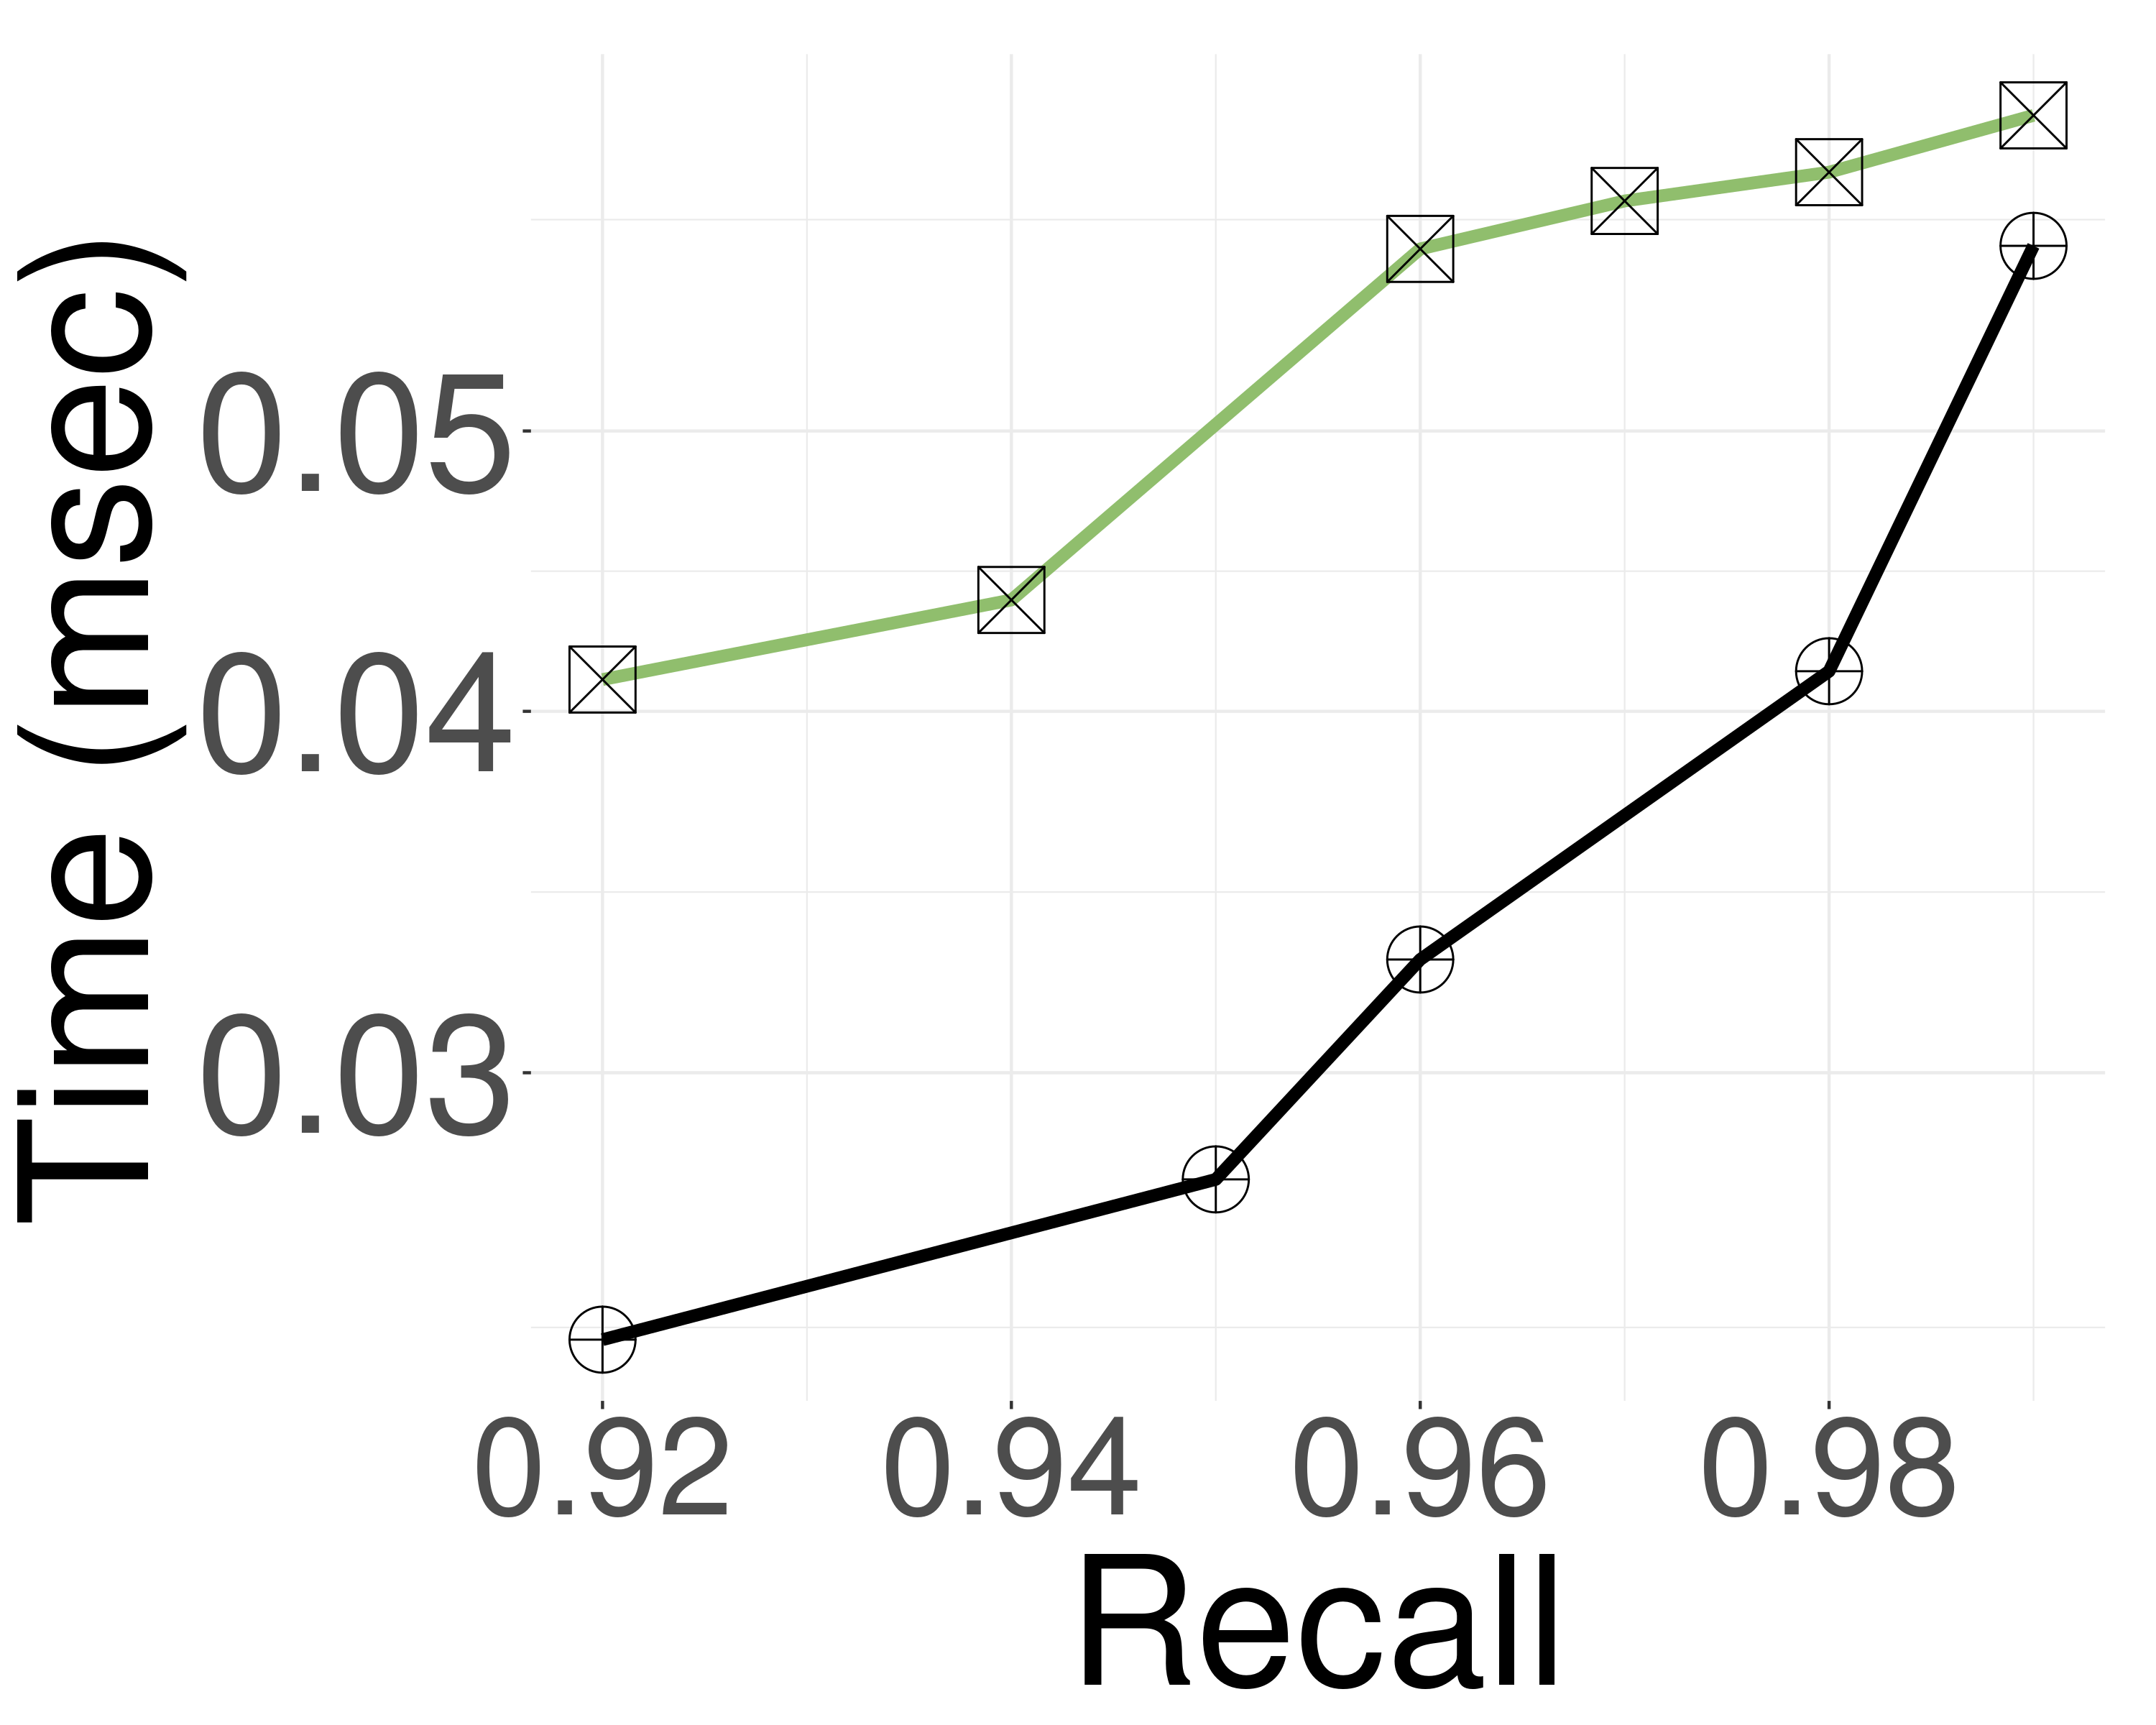
\includegraphics[width=0.4\columnwidth]{../img/elpis2/pre/deep_Time.png}
		\caption{Parallel batch query workload (Deep100GB)}       
		\label{fig:elpis2:pre}
 \end{figure}

Figure~\ref{fig:elpis2:pre}
 compares the performance of ELPIS on a batch query workload, where multiple queries are run in parallel (ELPISPMQS), to HNSW on the same setting (HNSWPMQS). We straightforwardly adapt both methods by assigning different queries to different threads. We remark that the performance of ELPIS on multiple queries lag behind that of HNSW. This is mainly due the fact that ELPIS assigns multiple threads to each query, while HNSW dedicates one thread to each query, thereby achieving a higher throughput.
 
To address this issue, we introduce two main changes to ELPIS for batch query workload scenario: i) we minimize the number of threads required to answer one query by increasing the maximum size of each leaf (originally set within 4-10\% of the dataset size); and ii) we disable the heuristic search which prunes non-promising leaves with EAPCA, as the total number of leaves decreases with the increase of leaf size.
%search all leaves at one time instead of running the search on approximate leaf and pruning the non promissing leaves with EAPCA lb distance. 

\noindent{\textbf{Minimize the number of threads needed by each query.}} ELPIS answers each query by searching multiple leaves in parallel. Thus, to maximize the number of queries that can be answered within a time interval, we should minimize the number of threads used by each query. 
%during parallel multi-queries search, we dedicate a set of threads for each query, then answer the different queries divide the number of available threads by the number of threads required to answer each query, then asearch on all leaves in parallel for each node. Thus to minimise the number of threads required for each query to run in one time, 
We can achieve the latter either by improving the pruning of leaves to have less promising leaves to search, or by increasing the maximum leaf size to have fewer candidate leaves to start with. We opted for the second option and found that setting the maximum leaf size to be 40\% the dataset size leads to the best performance. Nevertheless, the search efficiency was still not satisfying as we need to also adapt the search with the new maximum leaf size setting, thus, we directly calculate the distance between the query and all leaves and run search on \textit{nprobes} leaves with smallest distance to the query, instead of running a retrieving and approximate results from approximate leaf in a first stage before pruning and running the search on \textit{nprobes-1} leaves with warmed candidate set.

\noindent{\textbf{Modify the ELPIS search algorithm.}} With a large maximum leaf size, the maximum number of leaves to search to reach high recall is significantly reduced. Thus, some steps in the ELPIS search algorithm were no longer needed and were disabled. For instance, performing a filtering of the leaves based on the EAPCA lower-bounding distance was no longer as effective, so the EAPCA leaves were all searched in parallel.
%, as nd directly run search on nprobes leaves with minimum distances, instead of running search on approximate leaves and prune the non promissing leaves before runing search on selected promissing leaves.

We applied these modifications to the ELPIS search algorithm, and refer to this new variant as ELPISPMQS.
%of ELPIS original implementation, and we refer to this new  We evaluate the performance of ELPIS with these modifications. We adapt the new setting, and test 
We evaluate its performance against HNSW on the Sift and Deep datasets (sizes 100GB and 1B). Our experiments show that the search performance of ELPIS-PMQS is now better or equivalent to that of HNSW, contrary to ELPIS original search (Fig ~\ref{fig:elpis2:pre}). This is because ELPIS-PMQS now only needs to search 2-3 leaves on average to retrieve high-recall answers, compared 14-22 leaves in the case of ELPIS.




 \begin{figure}[!htb]
		\captionsetup{justification=centering}
		\captionsetup[subfigure]{justification=centering}
  	\centering
   			
\includegraphics[width=0.4\textwidth]{../img/elpis2/pre/legendpre.png}
      
        	\centering
		\begin{subfigure}{0.3\textwidth}
			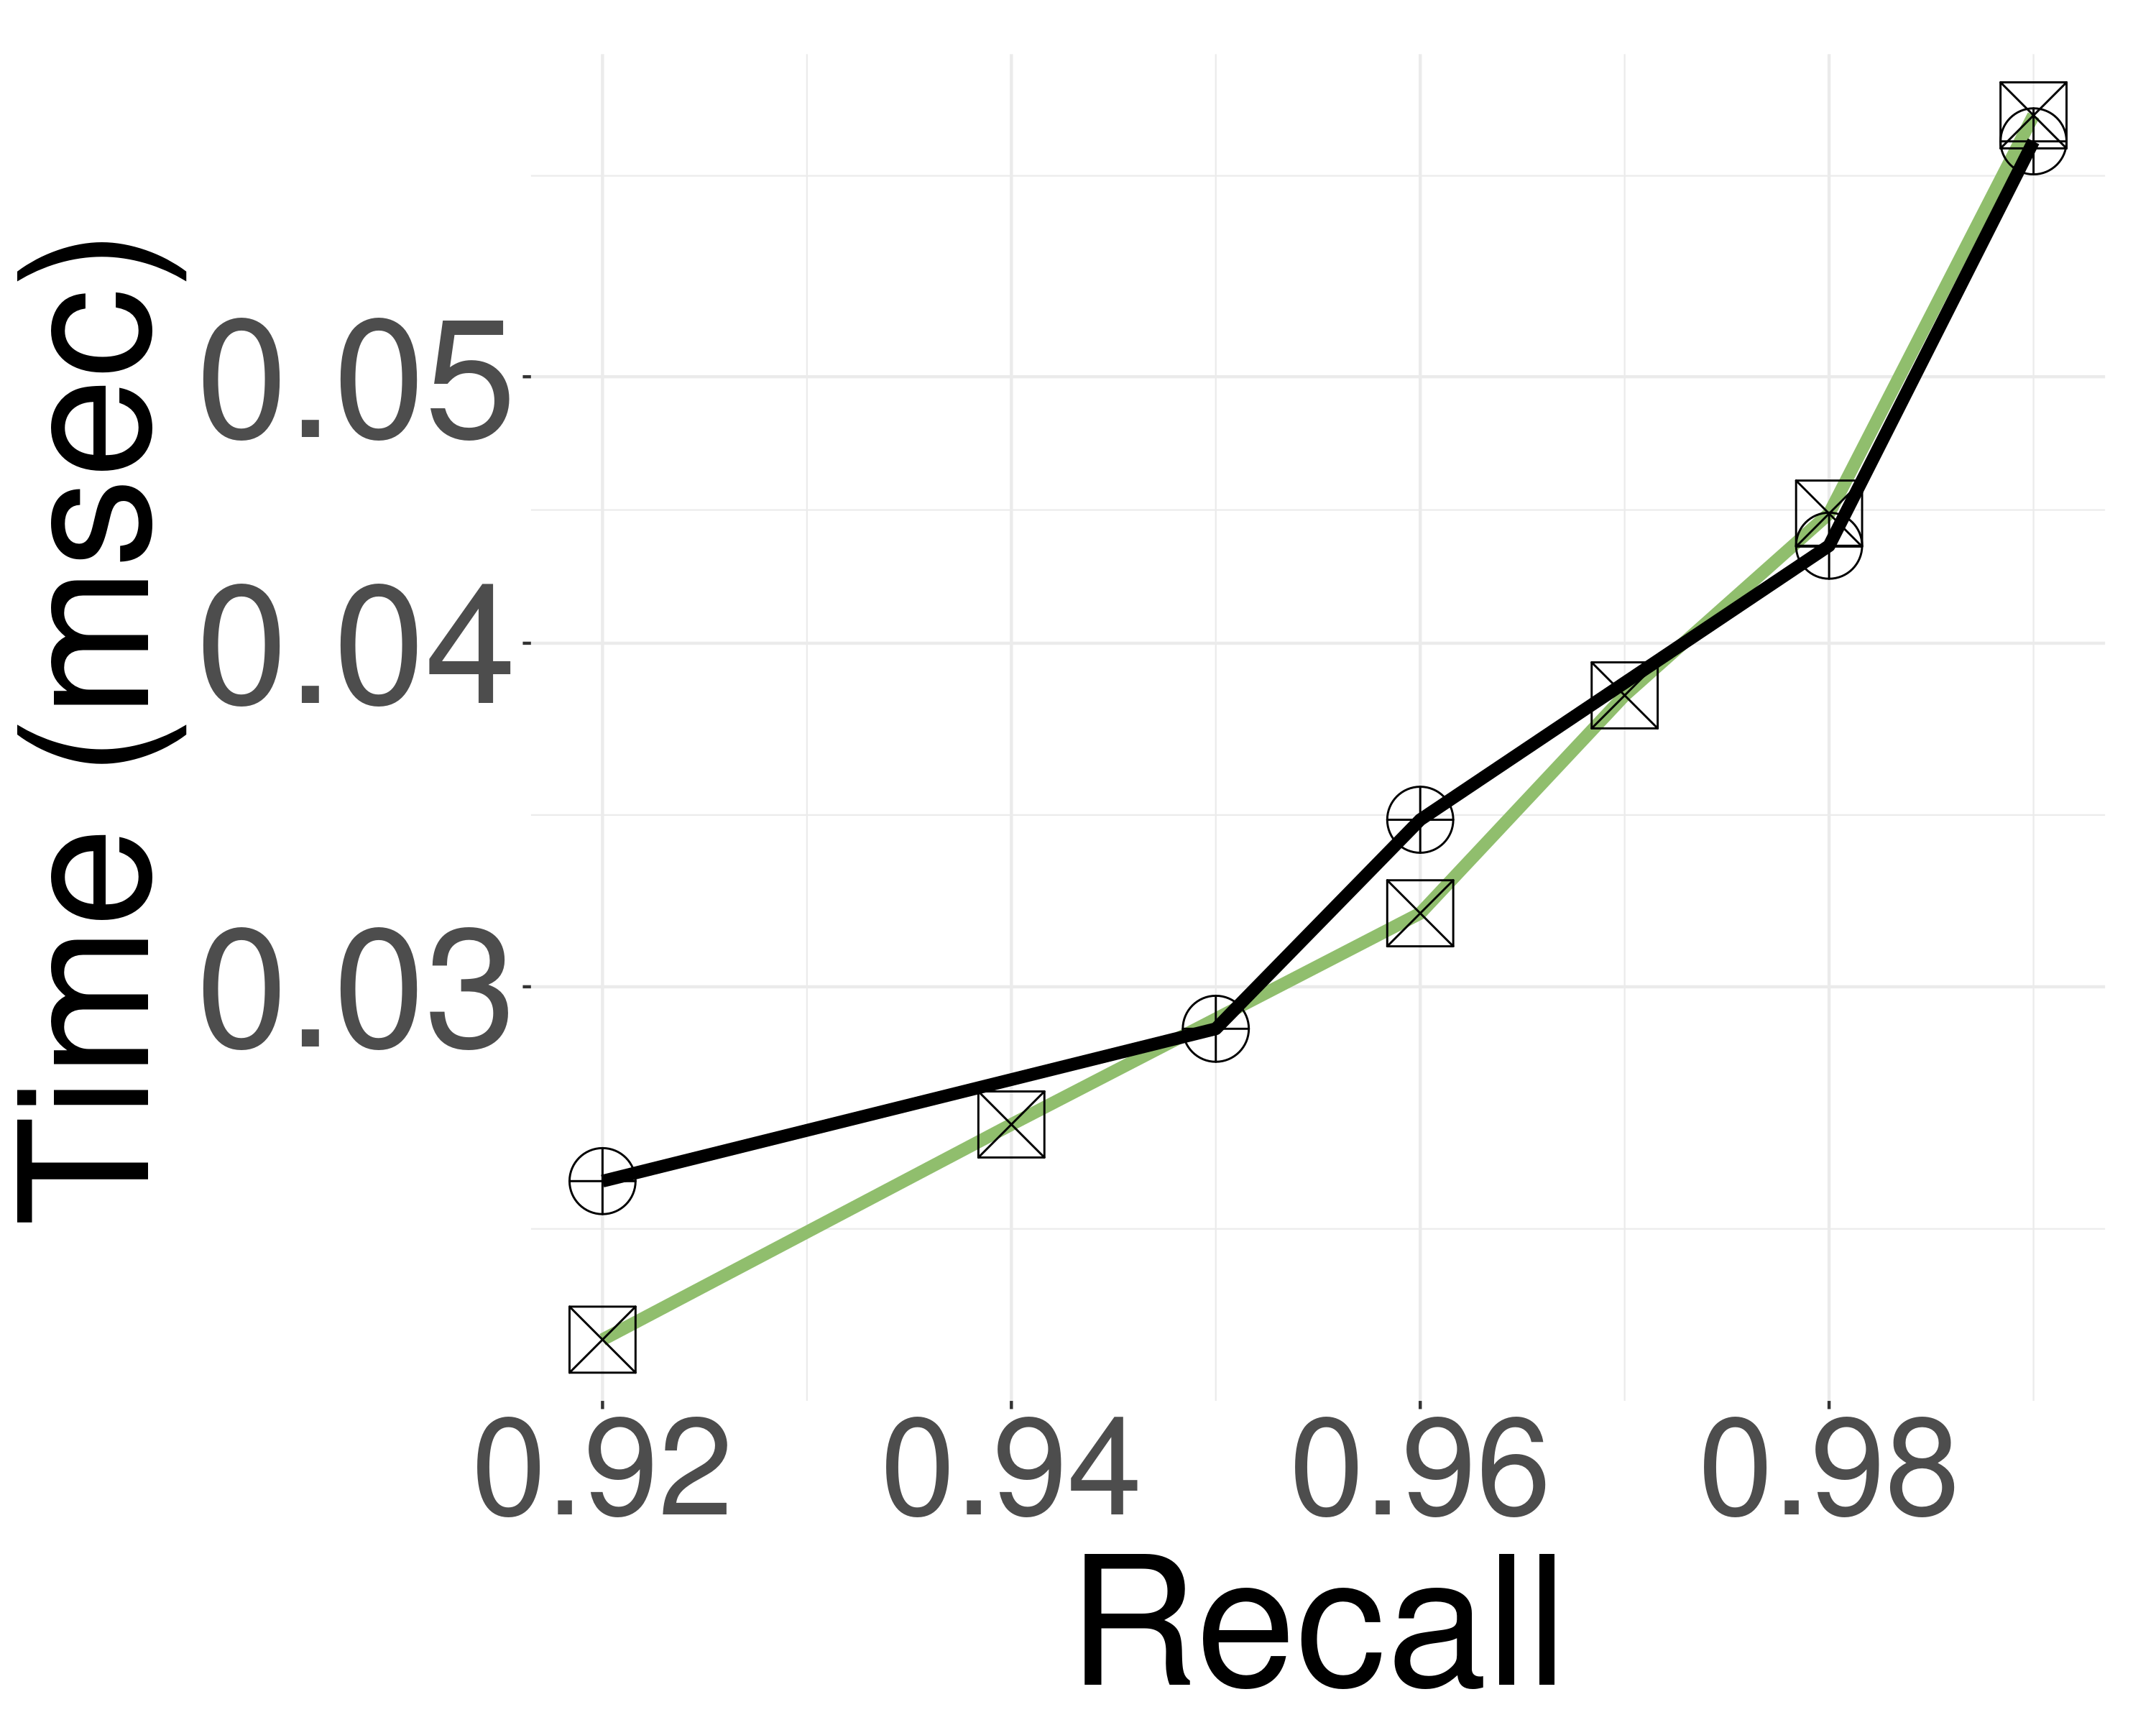
\includegraphics[width=\textwidth]{../img/elpis2/100GB/deep_Time.png}
			\caption{Deep}  
		\label{fig:elpis:query:performance:100GB:deep:10NN}
		\end{subfigure}
\hspace{0.4cm}
		\begin{subfigure}{0.3\textwidth}
			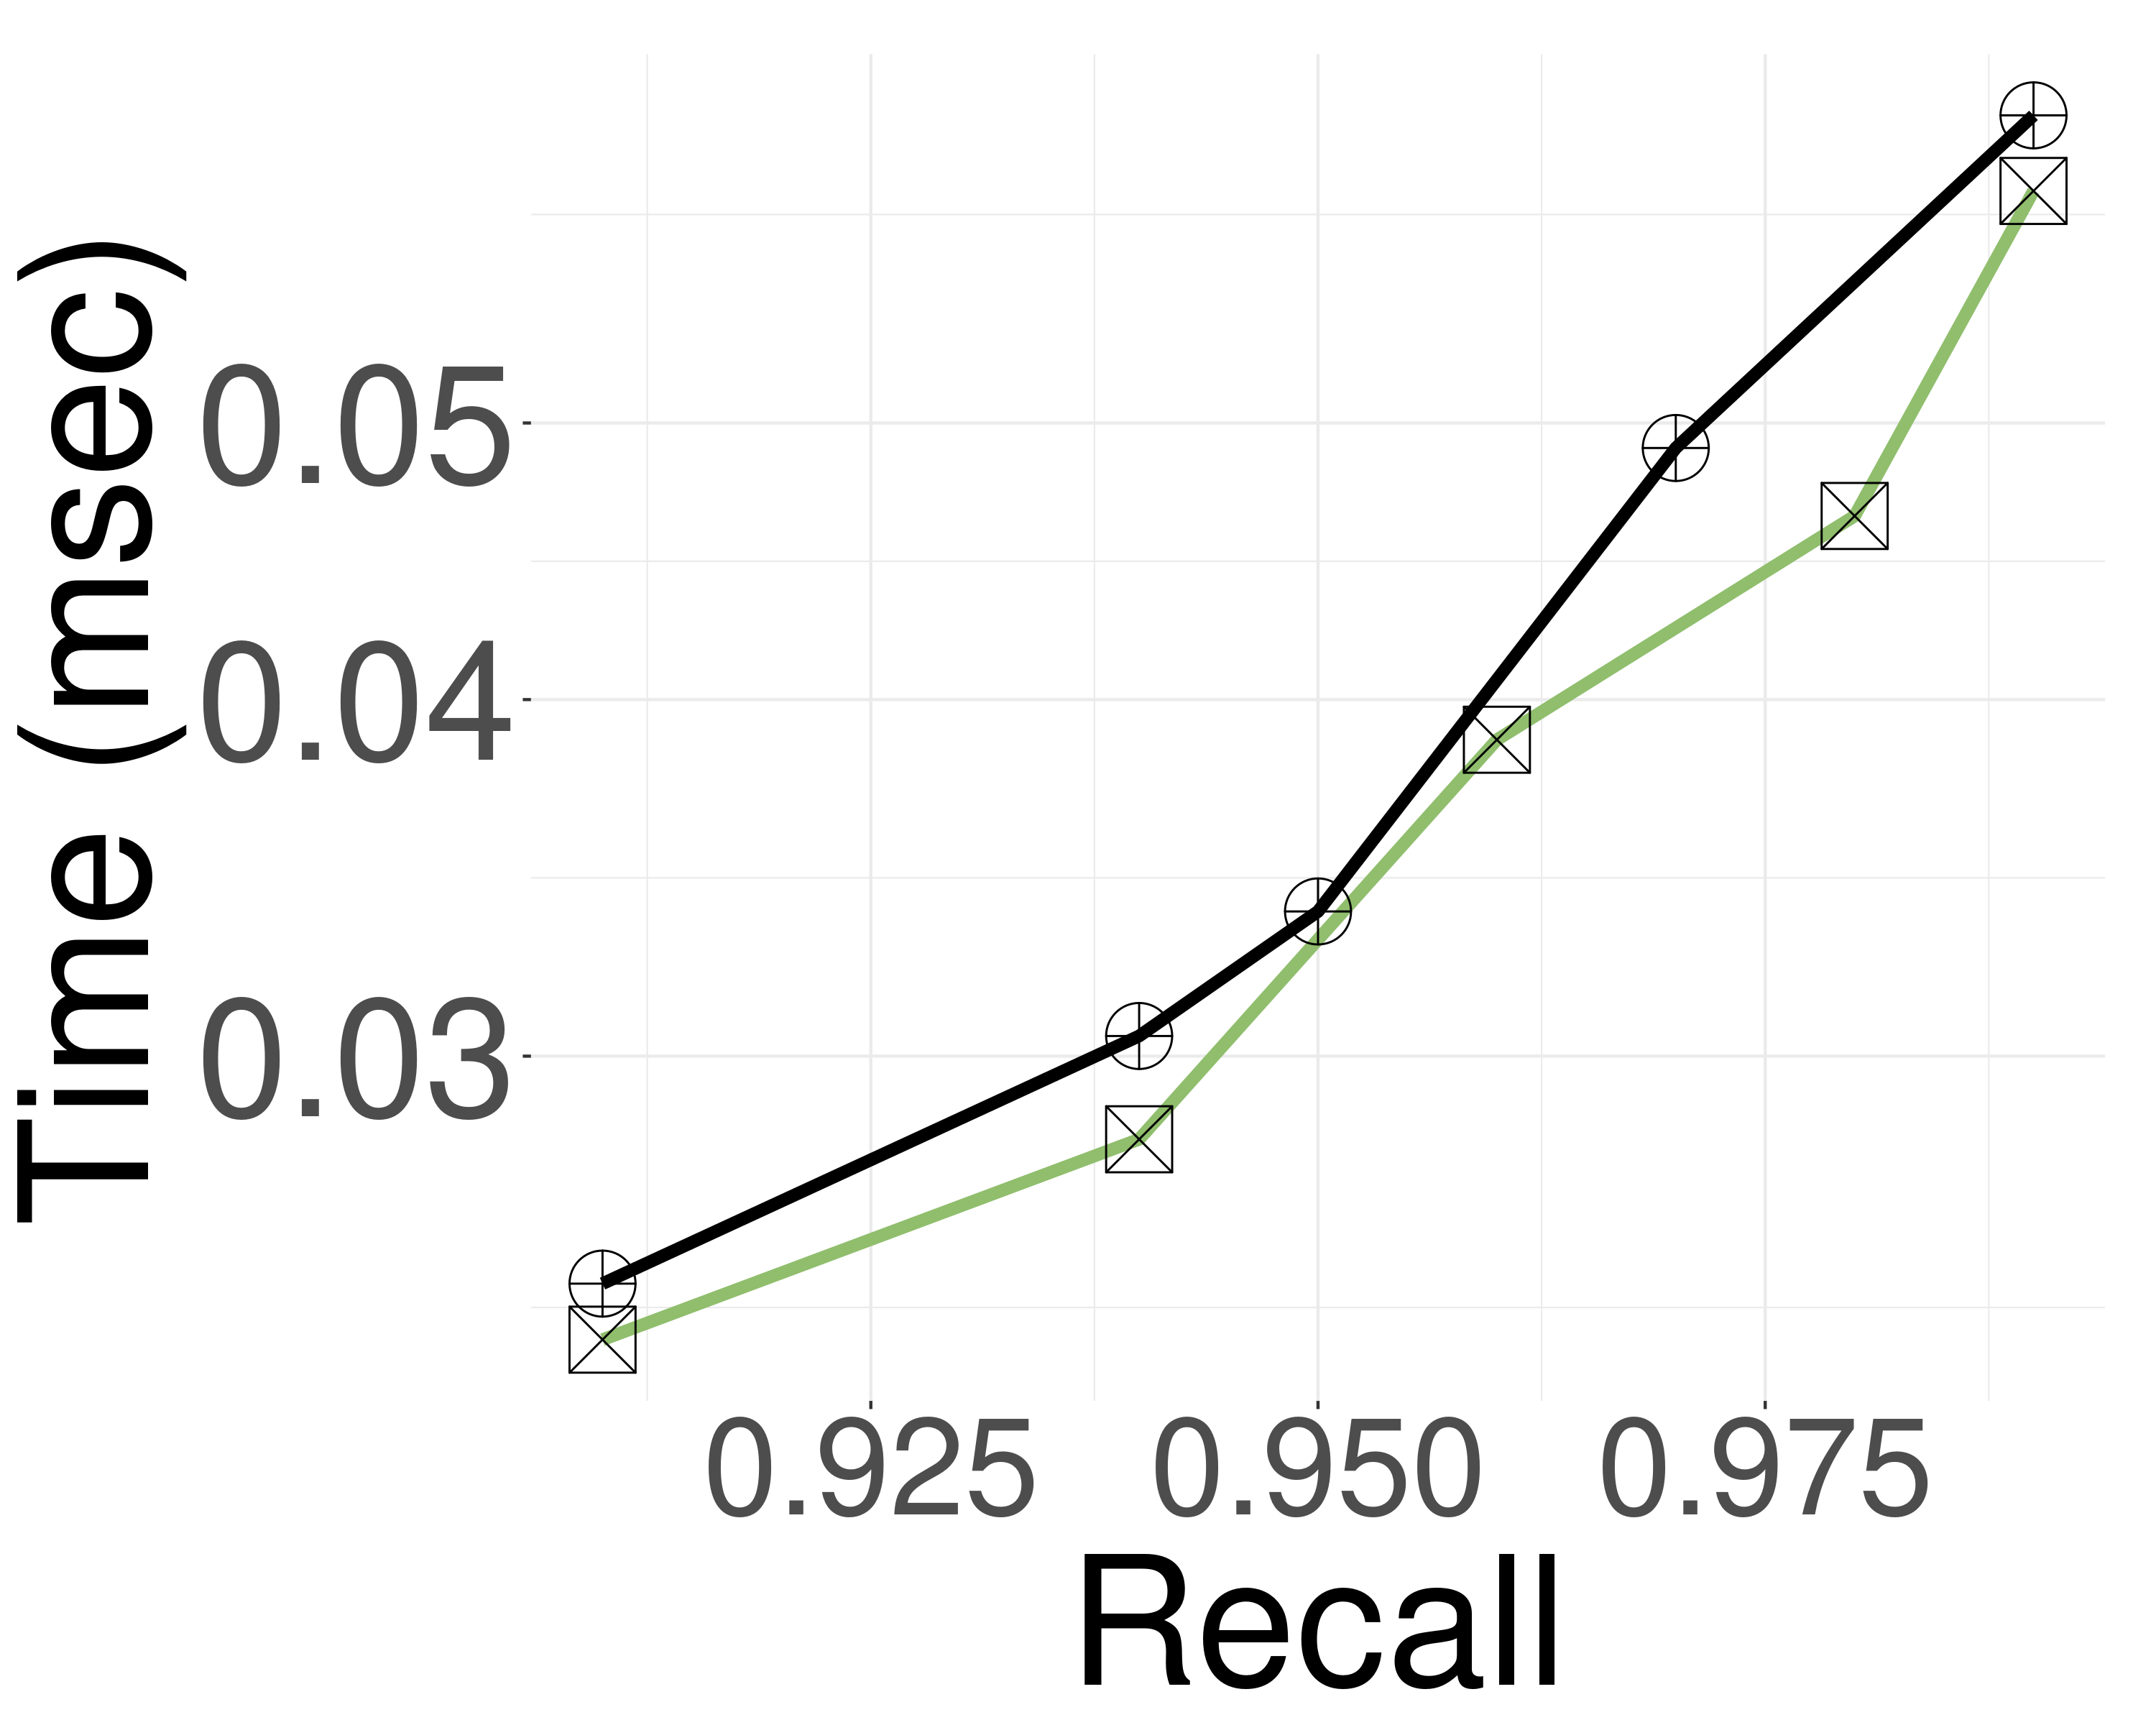
\includegraphics[width=\textwidth]{../img/elpis2/100GB/sift_Time.png}
			\caption{Sift}  
		\label{fig:elpis:query:performance:100GB:sift:10NN}
		\end{subfigure}
		\caption{{Search Performance on 100GB datasets}}	
		\label{fig:elpis2:nleafsize:100GB}
	\end{figure}
 
	\begin{figure}
		\captionsetup{justification=centering}
		\captionsetup[subfigure]{justification=centering}
  \centering
   			
\includegraphics[width=0.4\textwidth]{../img/elpis2/pre/legendpre.png}
  
  	\centering
		\begin{subfigure}{0.3\textwidth}
			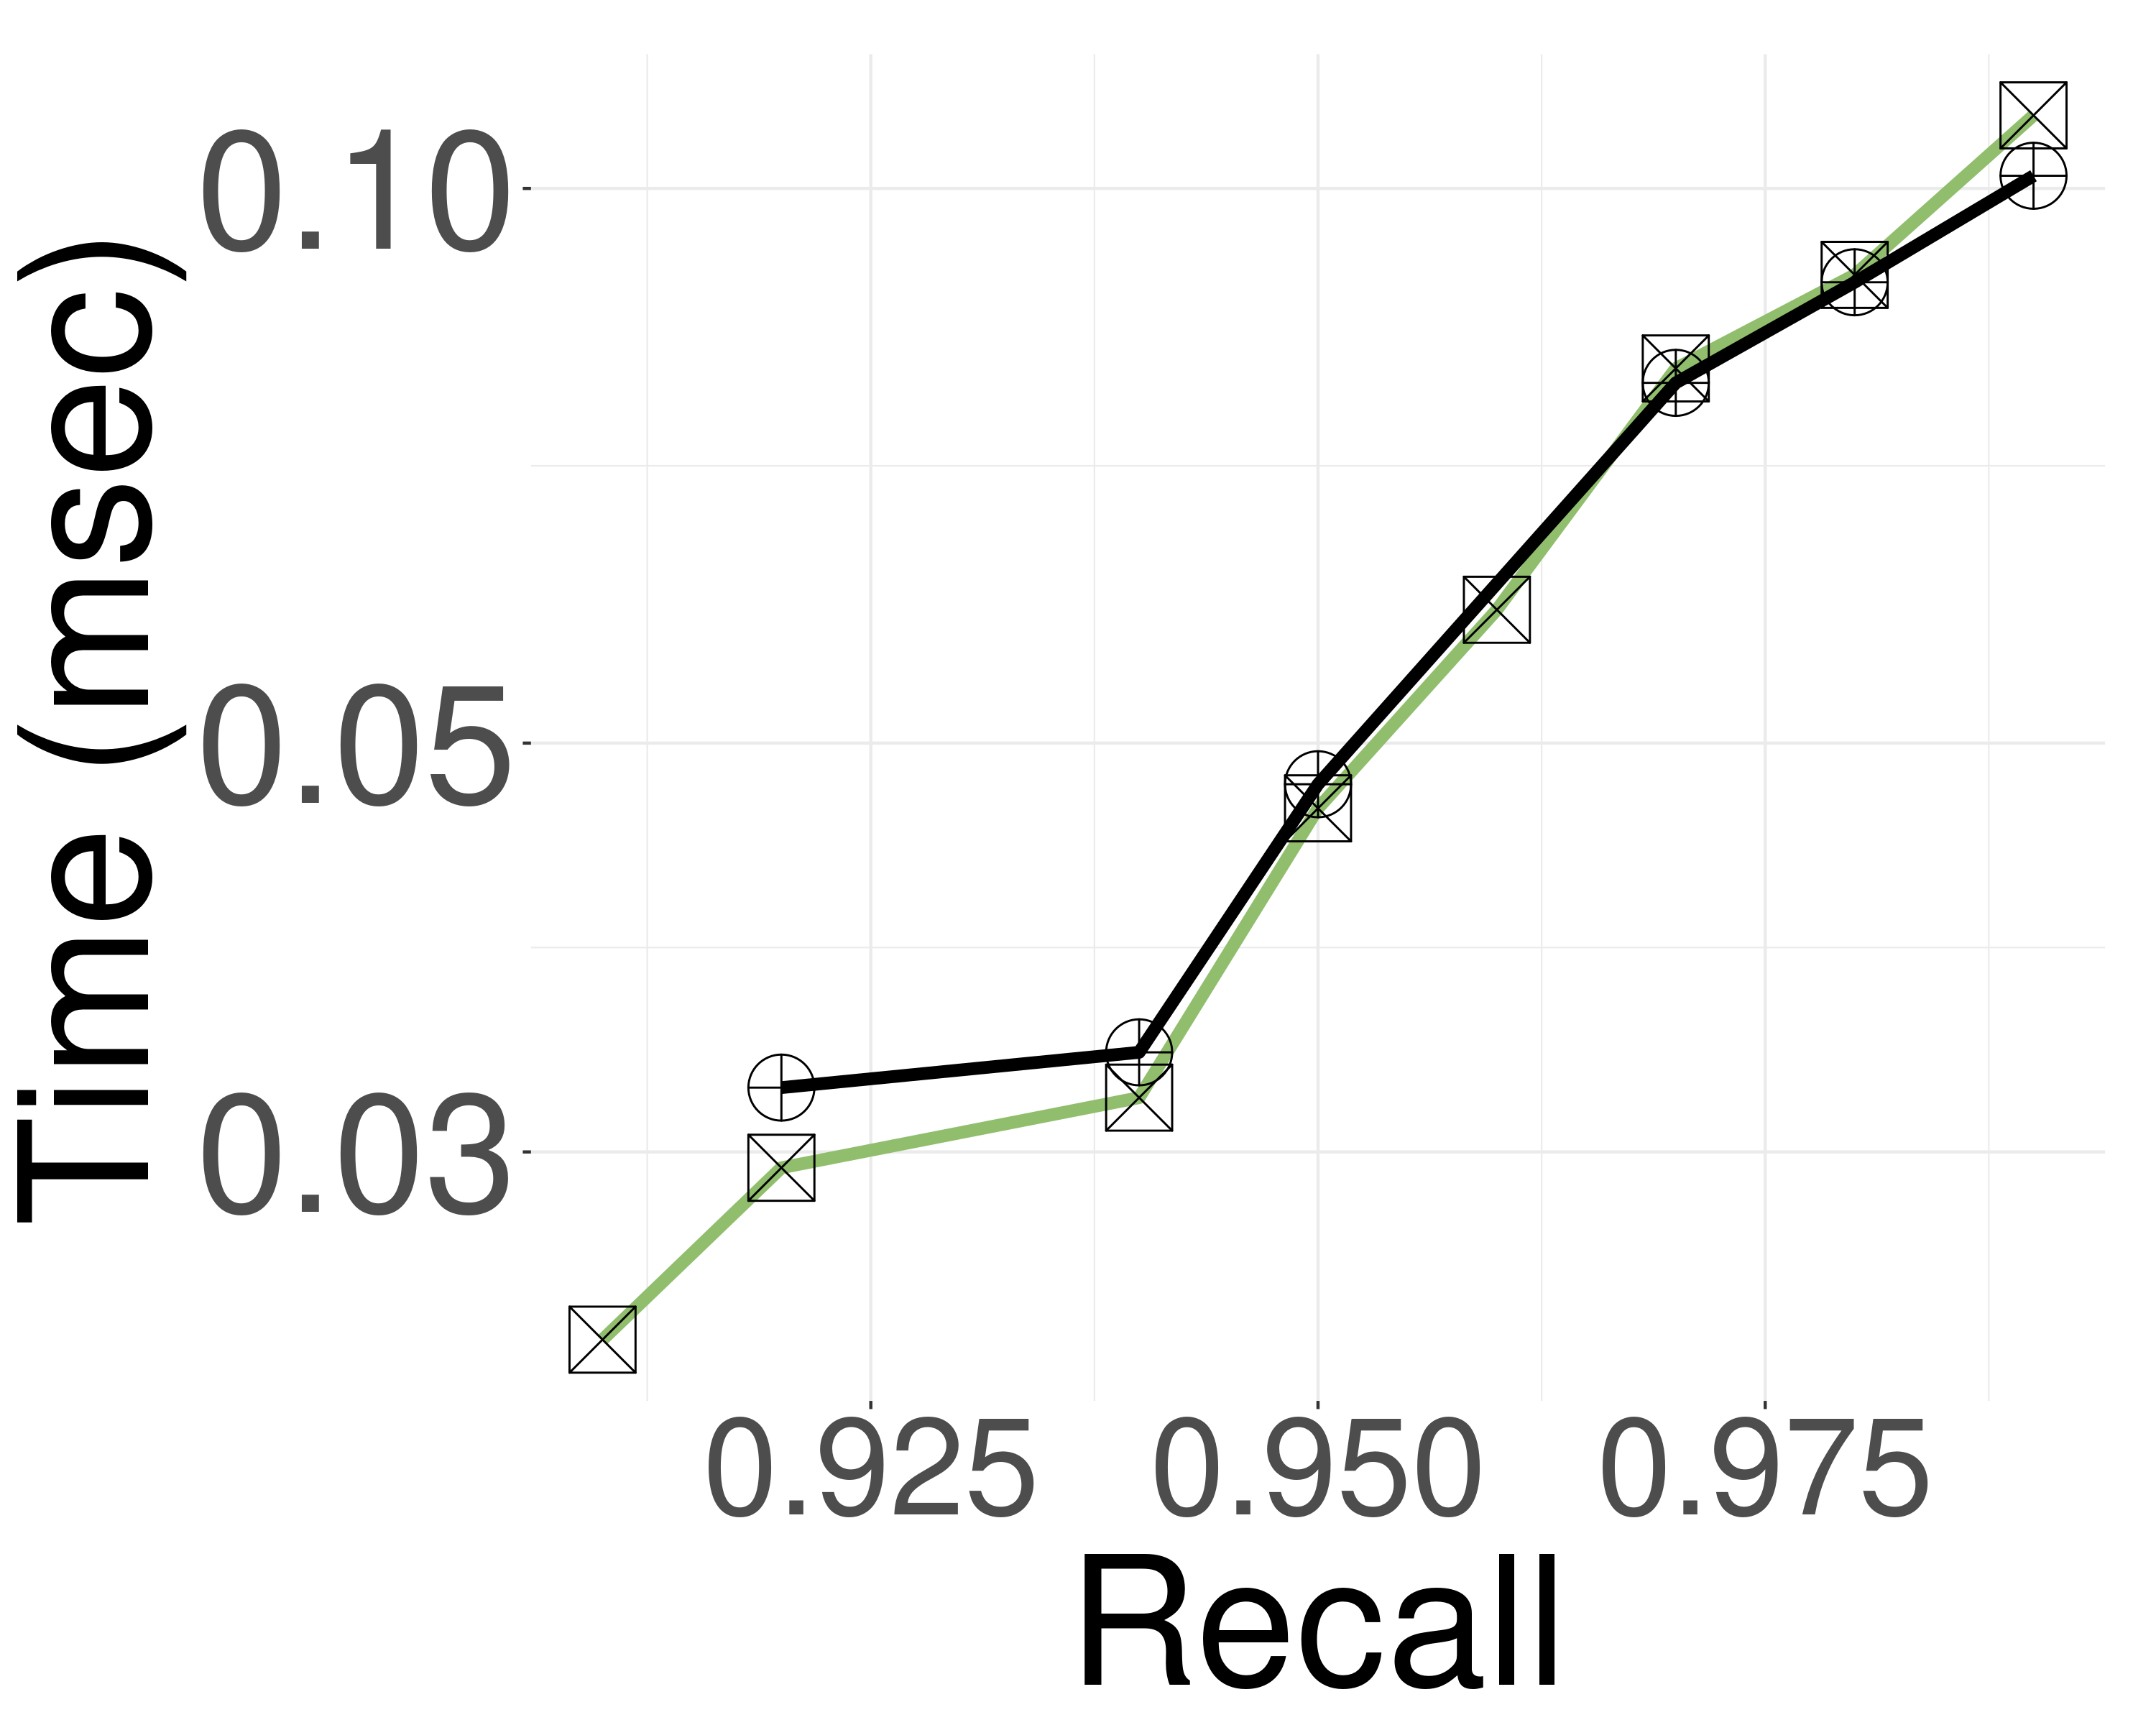
\includegraphics[width=\textwidth]{../img/elpis2/1B/deep_Time.png}
			\caption{Deep}  
		\label{fig:elpis:query:performance:1B:deep:10NN}
		\end{subfigure}
  \hspace{0.4cm}
		\begin{subfigure}{0.3\textwidth}
			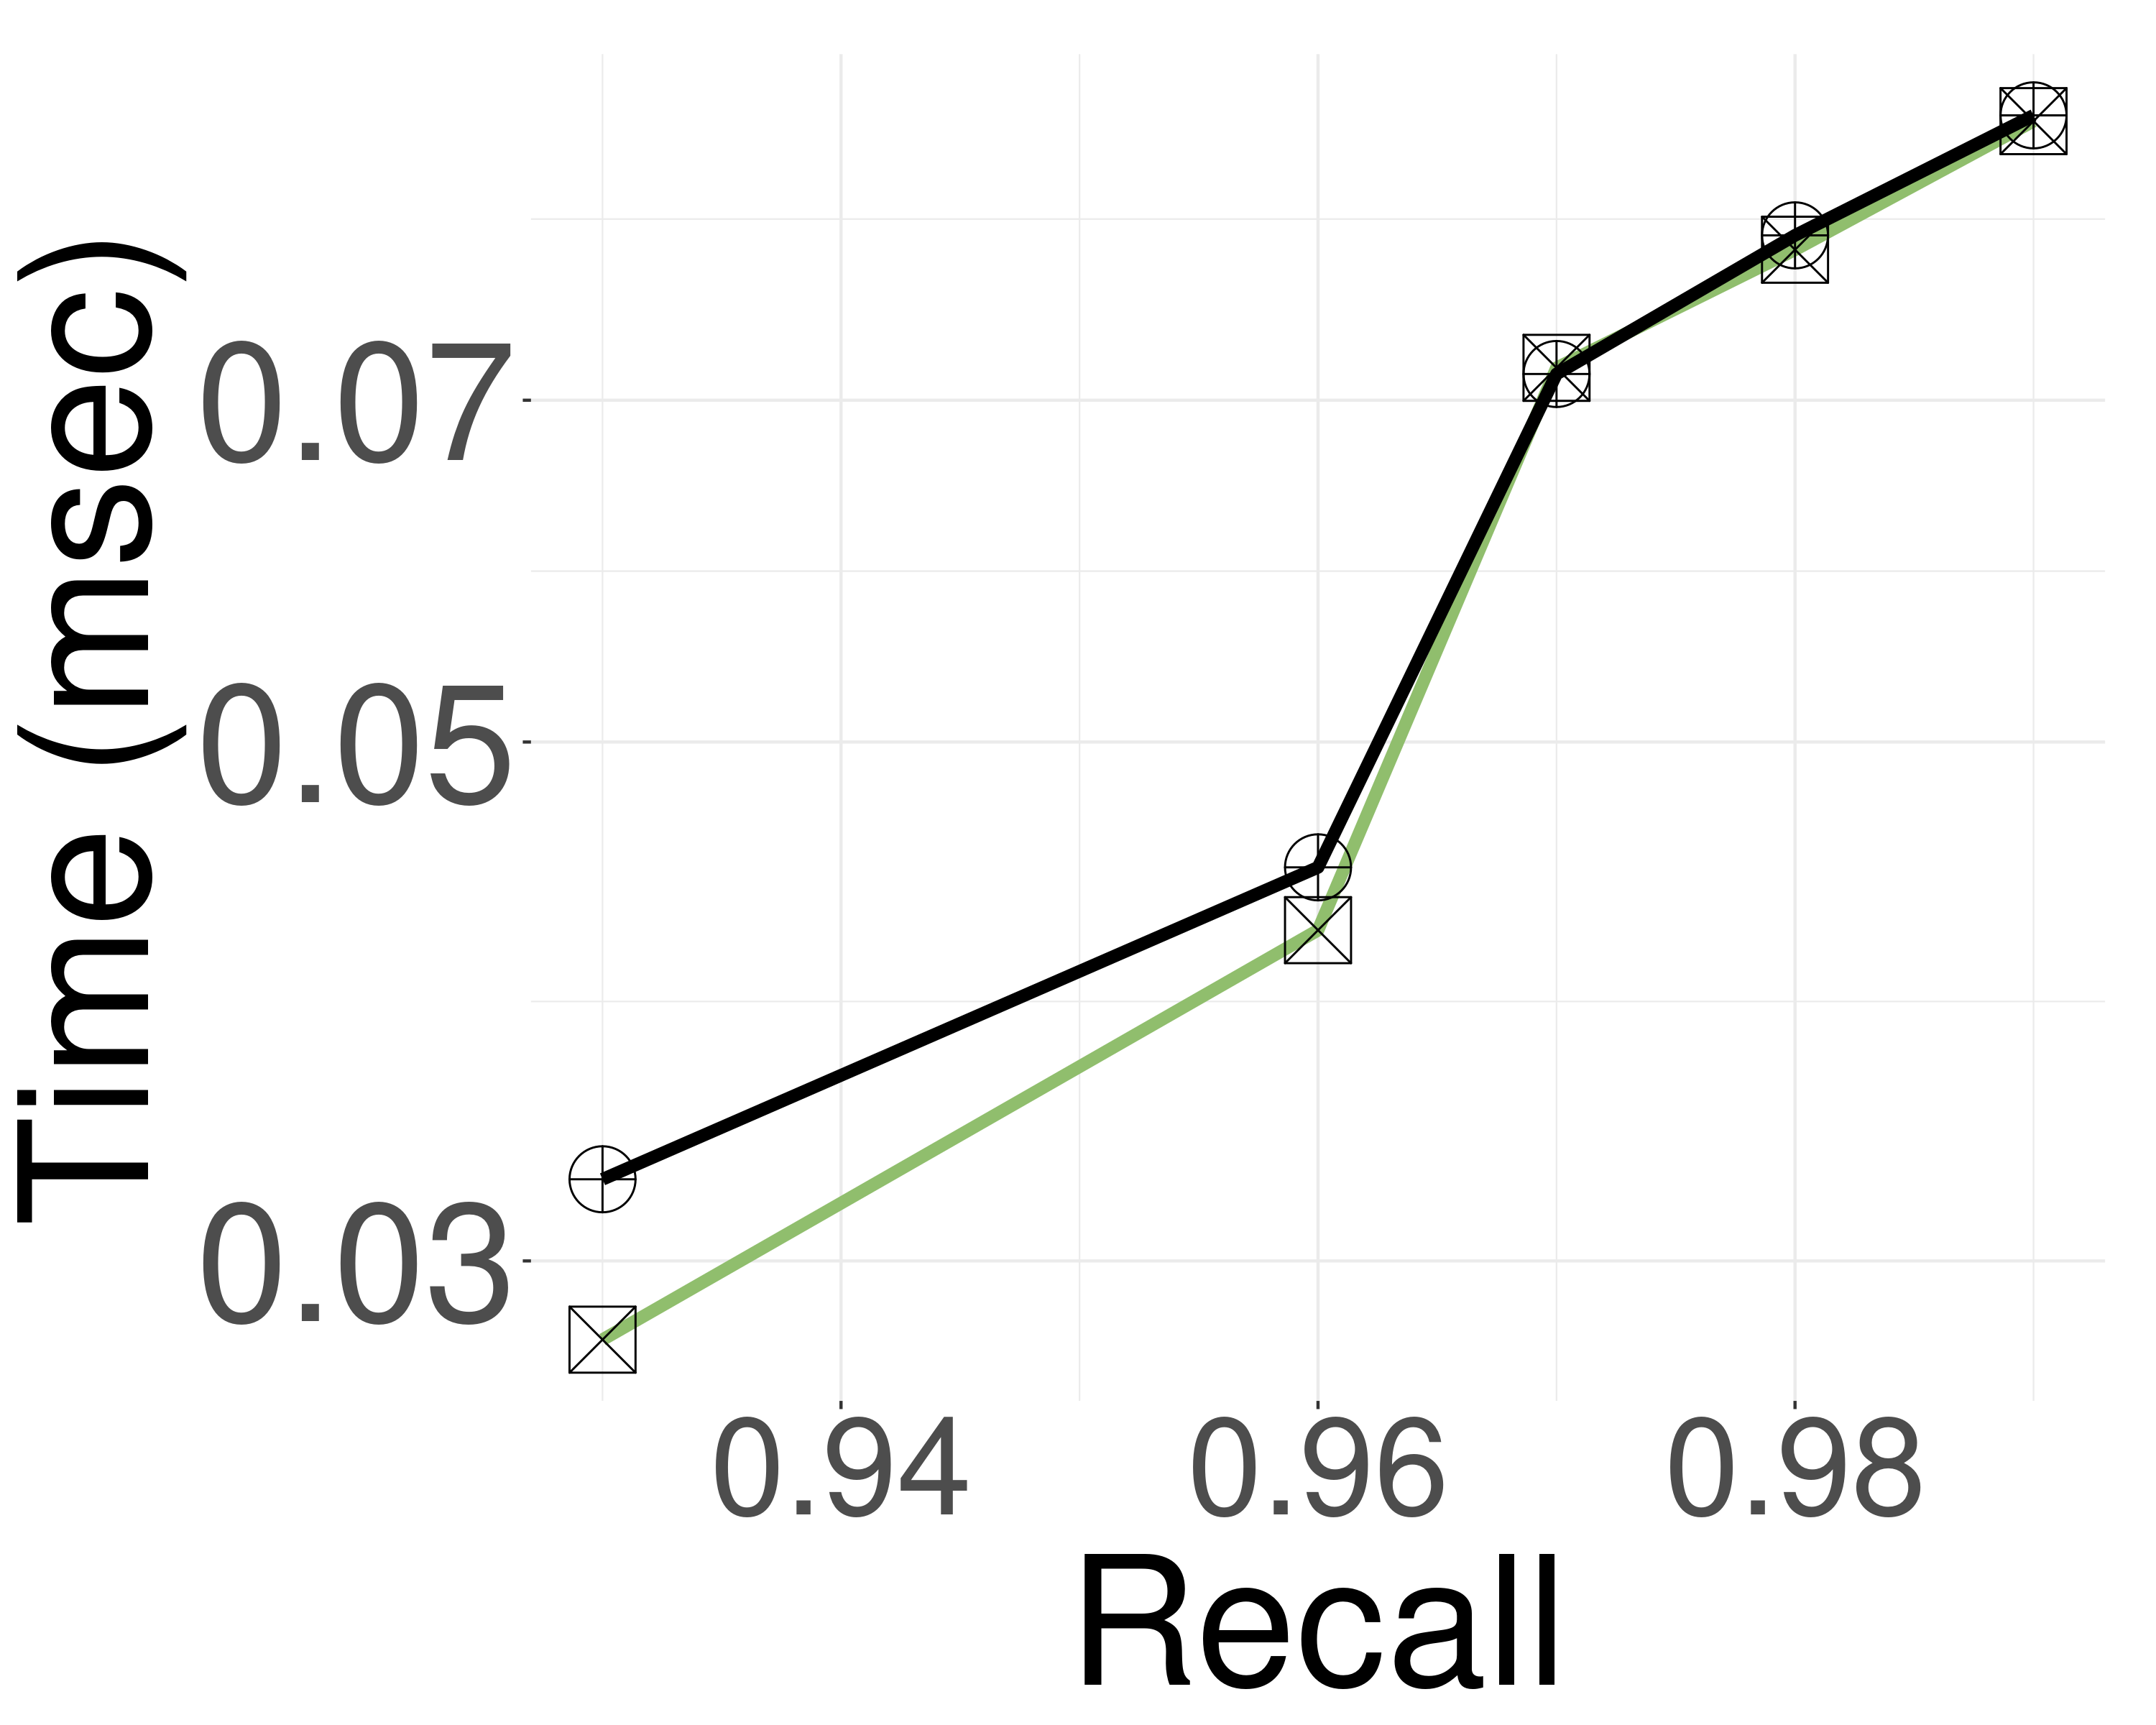
\includegraphics[width=\textwidth]{../img/elpis2/1B/sift_Time.png}
			\caption{Sift}  
			\label{fig:elpis:query:performance:1B:sift:10NN}
		\end{subfigure}
		\caption{{Search Performance on 1B datasets}}	
		\label{fig:elpis2:nleafsize:1B}
	\end{figure}



\section{EAPCA-based Merging for ELPIS}
We have demonstrated that ELPIS can achieve a superior search performance in latency-optimized workloads by building a hybrid data structure that exploits both trees and graphs. The tree index splits the dataset into multiple clusters, one cluster per leaf, and a separate graph is built on each leaf. During search, all graphs are searched in parallel, where one thread is dedicated to each leaf. The smaller the leaves, the faster are both indexing and search. Therefore, we typically build ELPIS to have the same number of leaves as the number of available threads. We have also shown that this configuration is not optimal for throughput since threads should be distributed across different queries, so we need to minimize the number of threads used by each query. 

A naive solution would be to build a separate ELPIS index for each scenario, i.e., one index with large leaves to increase throughput, and another index with small leaves to reduce latency. However, since building graph indexes is expensive both in time and footprint, we propose ELPIS+, an extension of ELPIS based on a novel graph merging strategy that transforms an index with small leaves into one with large leaves without rebuilding the graphs in the individual leaves. Thanks to this merging strategy, the ELPIS+ graph structure can then exploit the same index to efficiently support both latency and throughput optimized workloads with minimal space and time overhead.

%ELPIS+ exploits a novel graph merging stratefy In this section, we propose an efficient merging method for ELPIS leaves based on EAPCA, which enables transforming small leaves into larger ones without the need to rebuild the entire graph.
%This approach is designed to support parallel query answering while minimizing computational effort.

%\subsection{Motivation}


\subsection{EAPCA Merging Approach}

A straightforward merging strategy would retrieve, for any given internal node in the EAPCA tree, the graph nodes of all descendant leaves and construct a new graph on all the nodes. However, this approach is computationally expensive. Instead, we propose an approximation method that merges smaller leaves by selecting a subset of vertices from the descendant leaves. The key challenge is determining which vertices to select from the leaves to approximate the merged graph. We propose using the EAPCA's lower-bounding distance to identify the vertices that are near their parent tree nodes, particularly those near splitting boundaries. These boundary vertices serve as the connection points between different leaves. 
%Our method selects a subset of vertices from each descendant leaf based on their proximity to their parent tree nodes and merges them into a single graph. The idea is to sample vertices closest to the tree nodes at different levels (parent, grandparent) in the EAPCA tree. This process is repeated for all descendant leaves, and the final graph approximates the new merged leaf.


%that are closest to the boundaries of the EAPCA splitting points. These boundary vertices will likely form critical inter-leaf connections.


\subsection{Algorithm for EAPCA-based Merging}
To merge the leaves of ELPIS, we first identify the uppermost nodes in the EAPCA tree that satisfy the new maximum leaf size criterion. For each such node, we determine its descendant leaves and execute the EAPCA merging process to construct the new leaves. Algorithm~\ref{alg:eapca_merge} details the procedure for merging multiple descendant leaves of ELPIS into a single leaf. 

\begin{algorithm}[htb]
\caption{EAPCA-based Merging}
\label{alg:eapca_merge}
\begin{algorithmic}[1]
    \Require A set of descendant leaves $\mathcal{L}$ of a tree, where each leaf $L_i$ has an associated graph $G_i$
    \Ensure Merged graph $G_{\text{merged}}$
    \State Initialize an empty set of nodes: $\texttt{selectedVertices} \gets \emptyset$
    \ForAll{ $L_i \in \mathcal{L}$}
        \State \texttt{branch} \leftarrow  \texttt{getbranch}($L_i$)
        \ForAll{Inode $n$ in the \texttt{branch}}
            \State Calculate the EAPCA lower-bound distance between the vertices in $L_i$ and $n$
            \State Select the top $t$ vertices with the smallest distances, where $t = \dfrac{|L_i|}{2^{1 + d}}$
            \State Add the selected vertices to \texttt{selectednodes}
        \EndFor
    \EndFor
    \State Build graph $G'$ of \texttt{selectednodes}.
\State $G_{\text{merged}} \gets G' \cup \left( \bigcup_{G_i \in \mathcal{L}} G_i \right)$
    \State \Return $G_{\text{merged}}$
\end{algorithmic}
\end{algorithm}

The merging process is broken down into the following steps :


\begin{enumerate}
    \item \textbf{Branch Traversal:} For each descendant leaf, the algorithm retrieves the set of its ancestor internal nodes, up to the new leaf node (Line 1).
    \item \textbf{Vertex Selection:} For each descendant leaf $L_i$, we select a subset of its vertices that are closest to the ancestor internal nodes in the tree based on the EAPCA lower-bounding distance. 
    These vertices are the most critical for connecting leaves (Lines 2-8).
    Specifically, for each internal node $n$, we select $t$ closest vertices, where
\[
t = \frac{|L_i|}{2^{1 + d}},
\]
and $d$ represents the number of hops between the internal node $n$ and $L_i$. Thus, $t$ decreases as we ascend from $L_i$ to the root node. 

    \item \textbf{Graph Construction with RRND:} The selected vertices from all leaves are used to build a new incremental insertion-based graph (HNSW). During this construction, we prioritize connections between vertices from different original leaves by relaxing the pruning over these connections using RRND instead of RND (Line 10).
    \item \textbf{Final Merged Graph:} After constructing the new graph $G'$, we merge all graphs from descendant leaves in $\mathcal{L}$ with $G'$, where vertices from different descendant leaves are connected through edges constructed during the building of $G'$.
\end{enumerate}

\subsection{Advantages of EAPCA-based Merging}

The EAPCA-based merging approach provides several advantages:
\begin{itemize}
    \item \textbf{Scalability:} ELPIS can handle growing leaf sizes efficiently without requiring the reconstruction of the entire graph.
    \item \textbf{Efficiency:} The process of selecting only boundary vertices minimizes computation and efficiently approximates key proximity edges for the merging of different graphs.
    \item \textbf{Optimized Connectivity:} The application of RRND during graph construction ensures that the connections between different leaves are optimized, supporting efficient traversal between different regions.
\end{itemize}

By leveraging the EAPCA-based merging strategy, ELPIS can dynamically scale and adapt to different workloads,  while maintaining high query accuracy.
\subsection{Discussion}

In Figures~\ref{fig:elpisem:query:performance:100GB} and~\ref{fig:elpisem:query:performance:1B}, illustrate how the new version of ELPIS, called ELPISEM-PMQS performs against HNSW and ELPIS-PMQS %on EAPCA-Merged ELPIS indices for
on the Deep and Sift datasets (sizes 100GB and 1B). ELPISEM-PMQS achieves comparable search performance to ELPIS-PMQS, the ELPIS index built from scratch with the same maximum leaf size on both the Deep and Sift 100GB datasets (Fig.~\ref{fig:elpisem:query:performance:100GB}). However, on the 1B-scale datasets, the merged indices struggle to deliver similar search efficiency. On both Deep and Sift 1B datasets (Fig.~\ref{fig:elpisem:query:performance:1B}), ELPISEM-PMQS requires extra distance calculations on the merged indices compared to ELPIS-PMQS without merging. This decrease in search efficiency is due to the absence of some promising edges for query answering between vertices from different original leaves.

 \begin{figure}[!htb]
				\captionsetup{justification=centering}
  
\includegraphics[width=0.6\textwidth]{../img/elpis2/EM/legendem.png}
		\captionsetup[subfigure]{justification=centering}
  	\centering
   
		\begin{subfigure}{0.3\textwidth}
			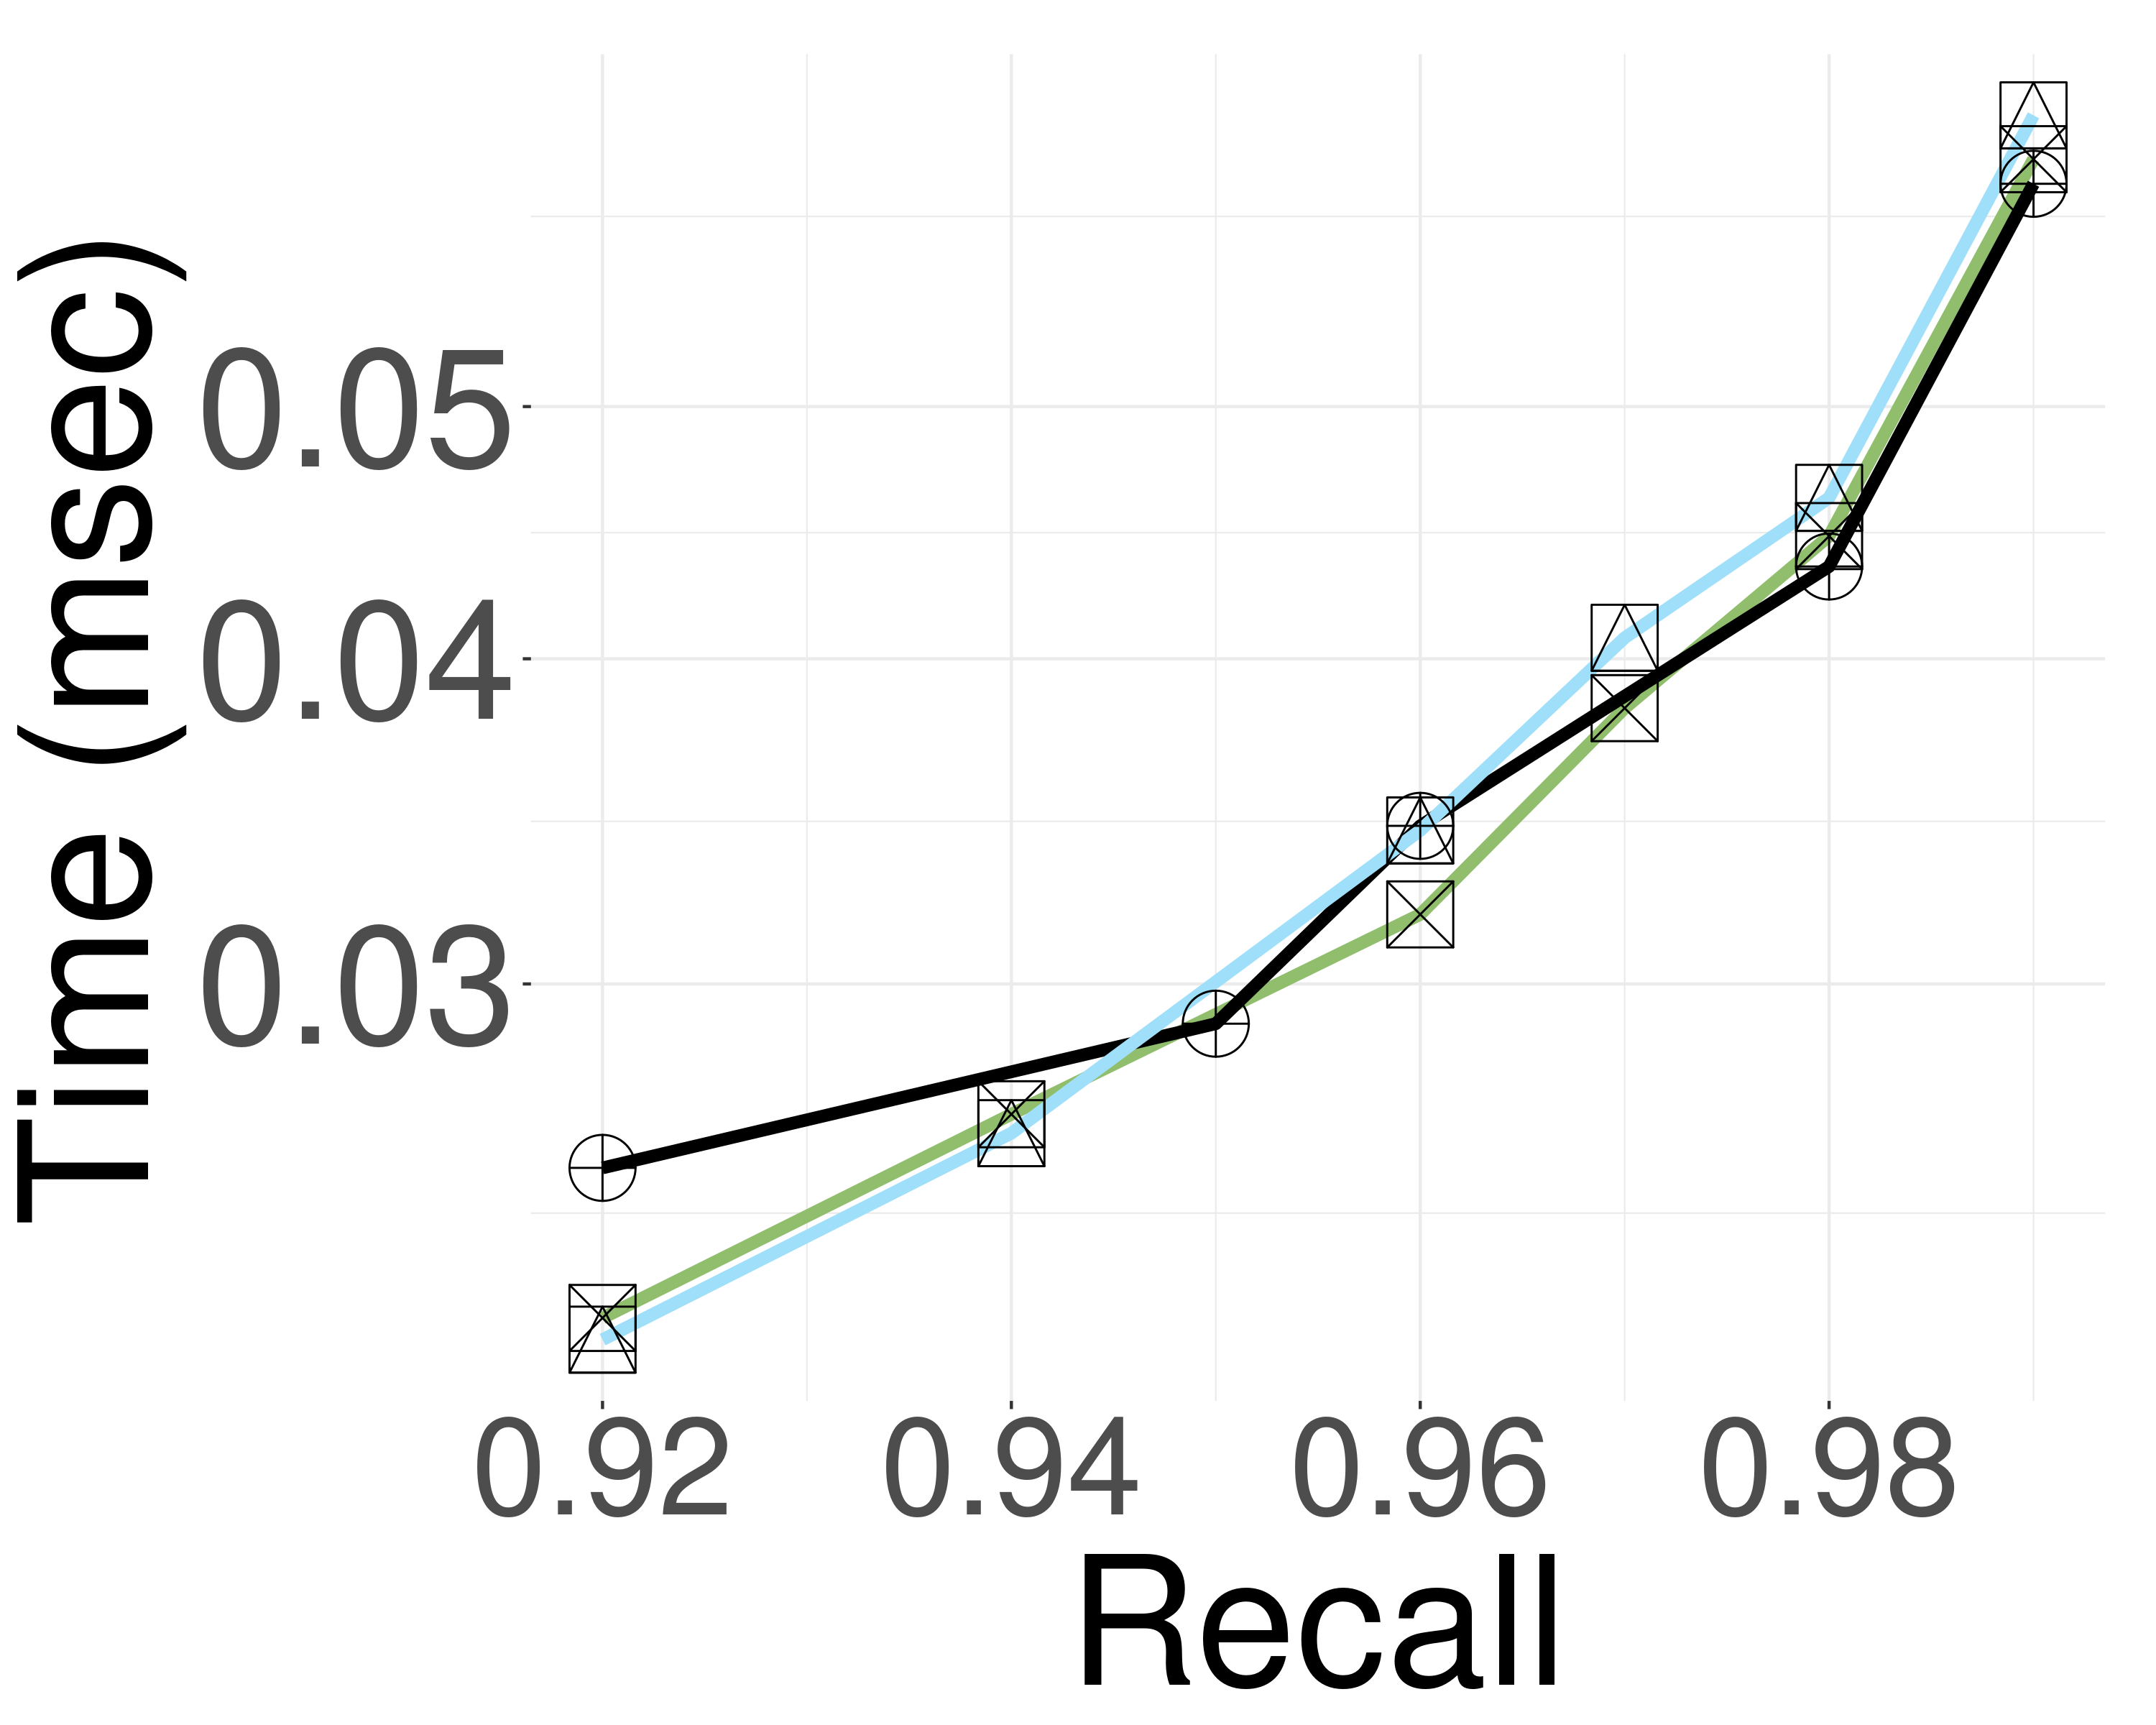
\includegraphics[width=\textwidth]{../img/elpis2/EM/100GB/deep_Time.png}
			\caption{Deep}  
		\label{fig:elpisem:query:performance:100GB:deep:10NN}
		\end{subfigure}
  \hspace{0.4cm}
		\begin{subfigure}{0.3\textwidth}
			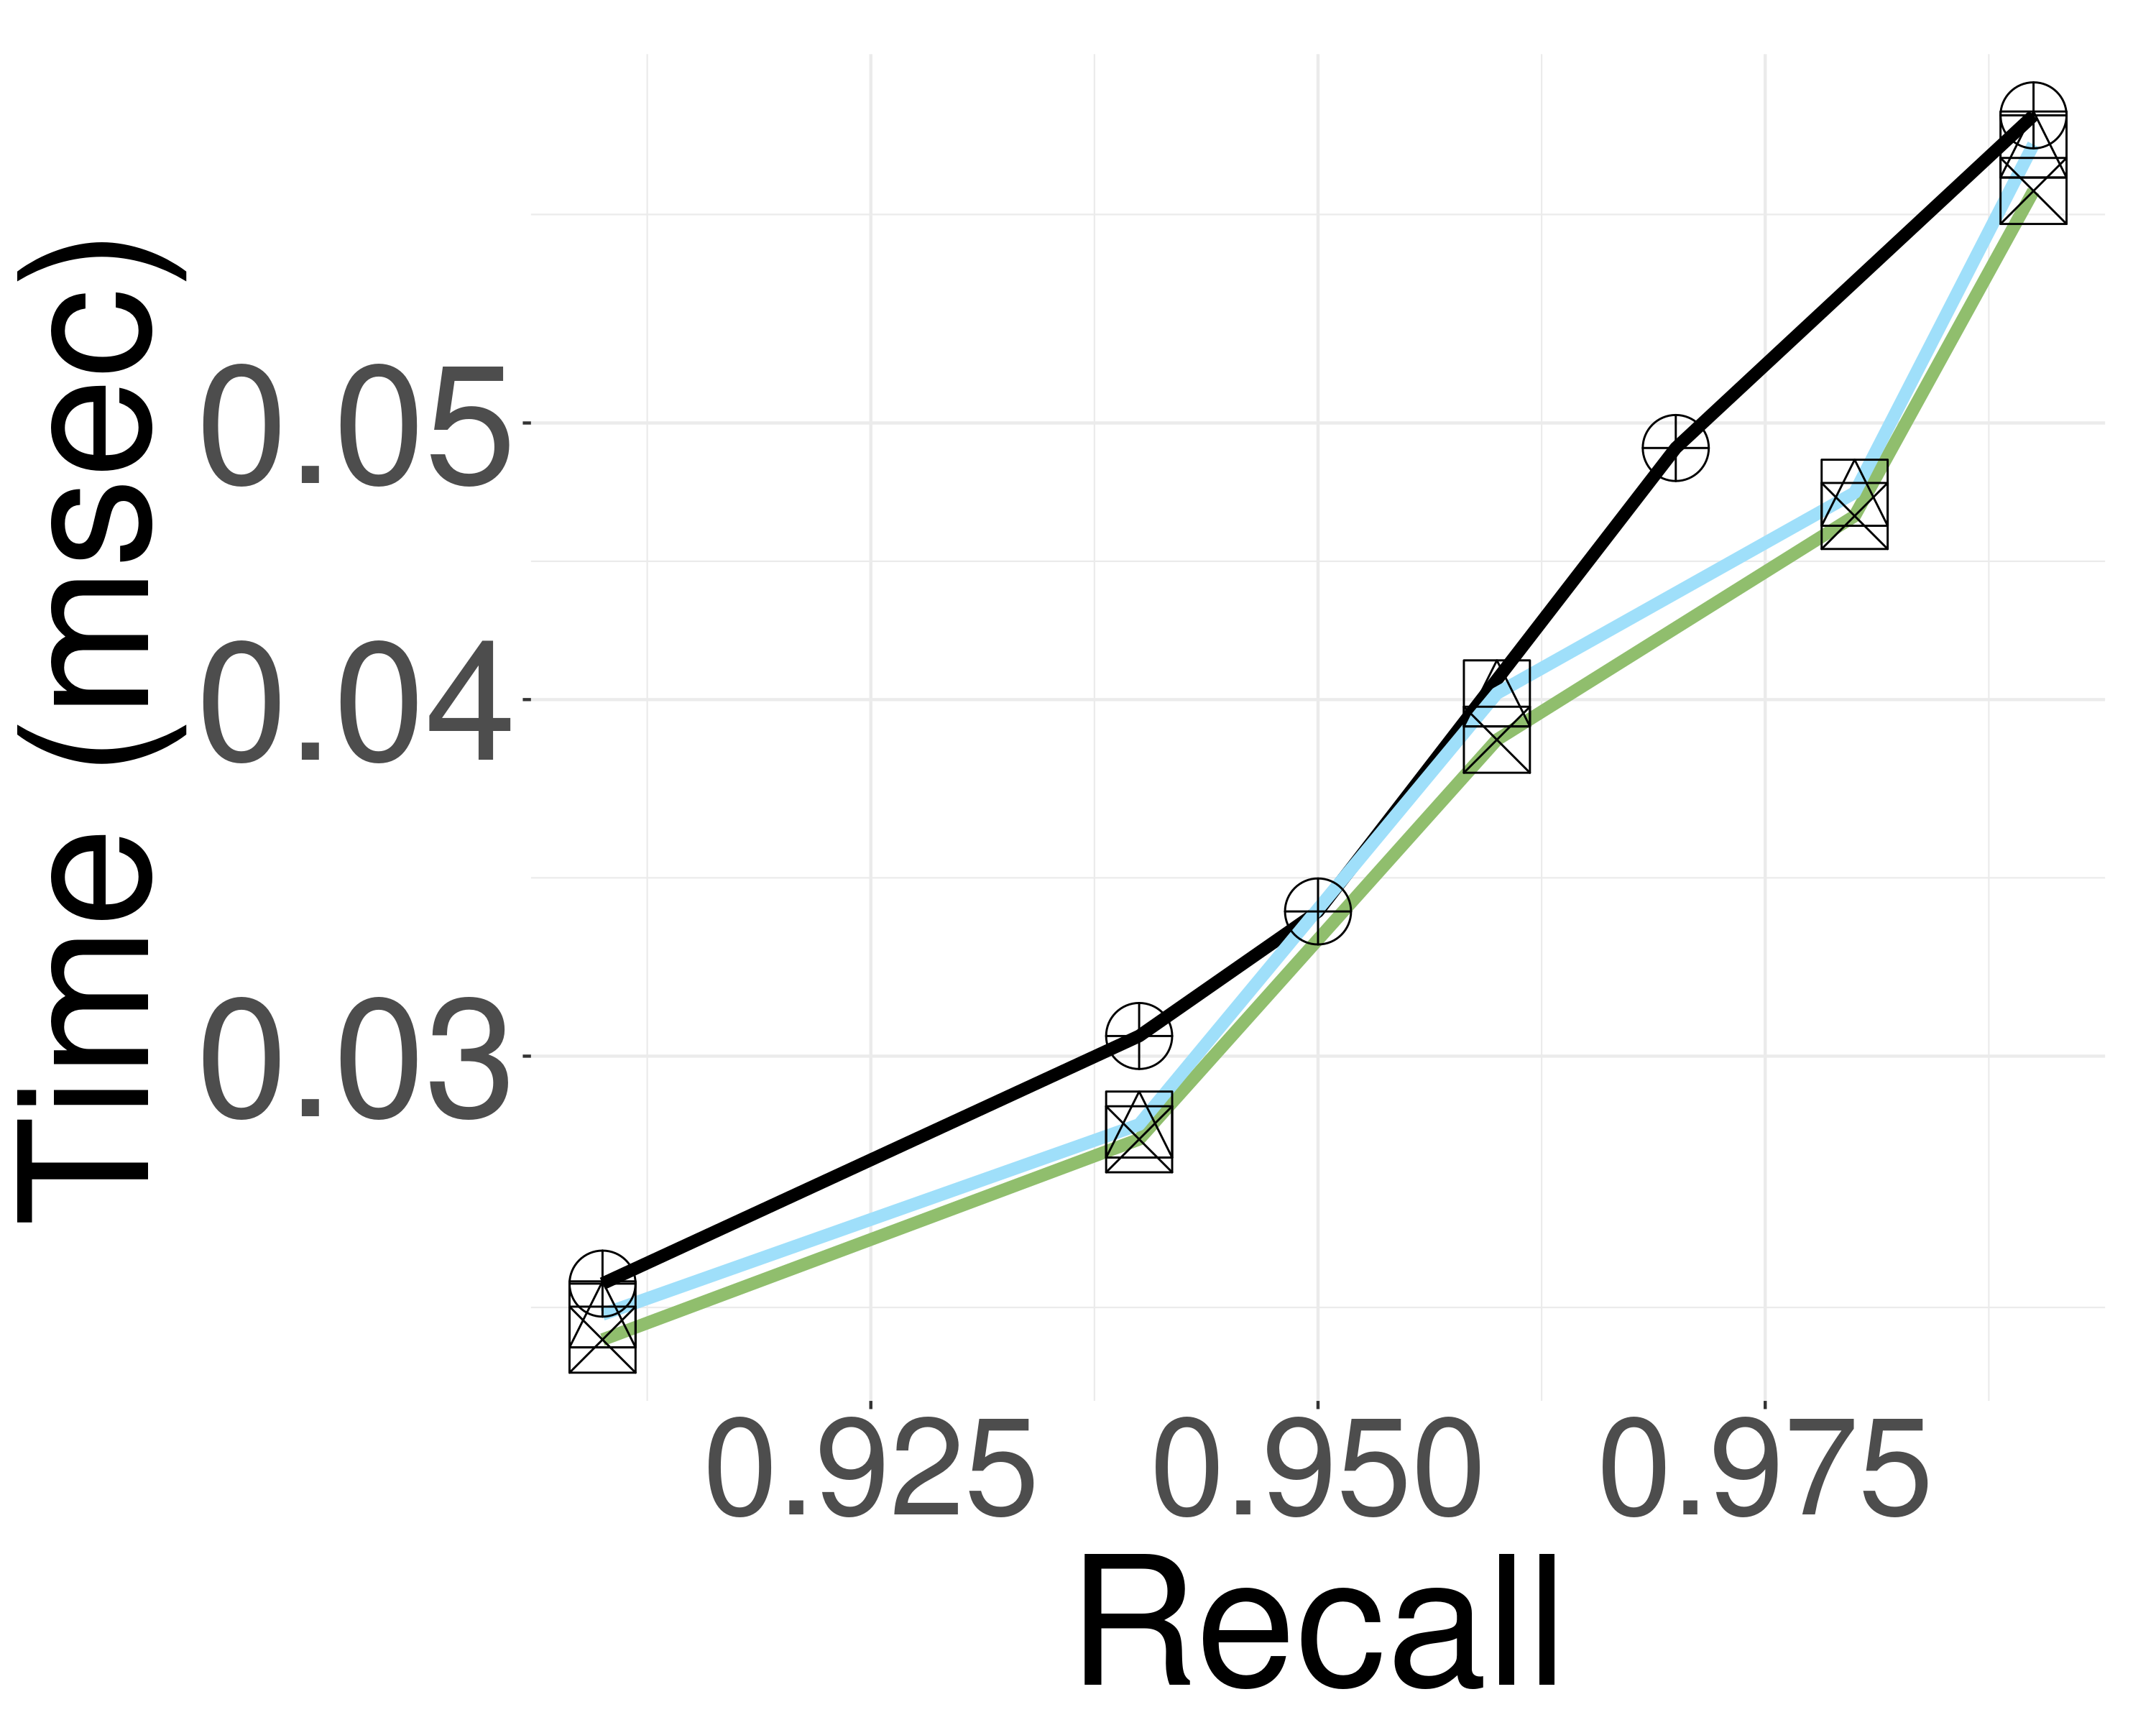
\includegraphics[width=\textwidth]{../img/elpis2/EM/100GB/sift_Time.png}
			\caption{Sift}  
		\label{fig:elpisem:query:performance:100GB:sift:10NN}
		\end{subfigure}
		\caption{{Search Performance on 100GB datasets}}	
		\label{fig:elpisem:query:performance:100GB}
	\end{figure}
 
	\begin{figure}
		\captionsetup{justification=centering}
  \centering
  
\includegraphics[width=0.6\textwidth]{../img/elpis2/EM/legendem.png}
  
		\captionsetup[subfigure]{justification=centering}
  	\centering
		\begin{subfigure}{0.3\textwidth}
			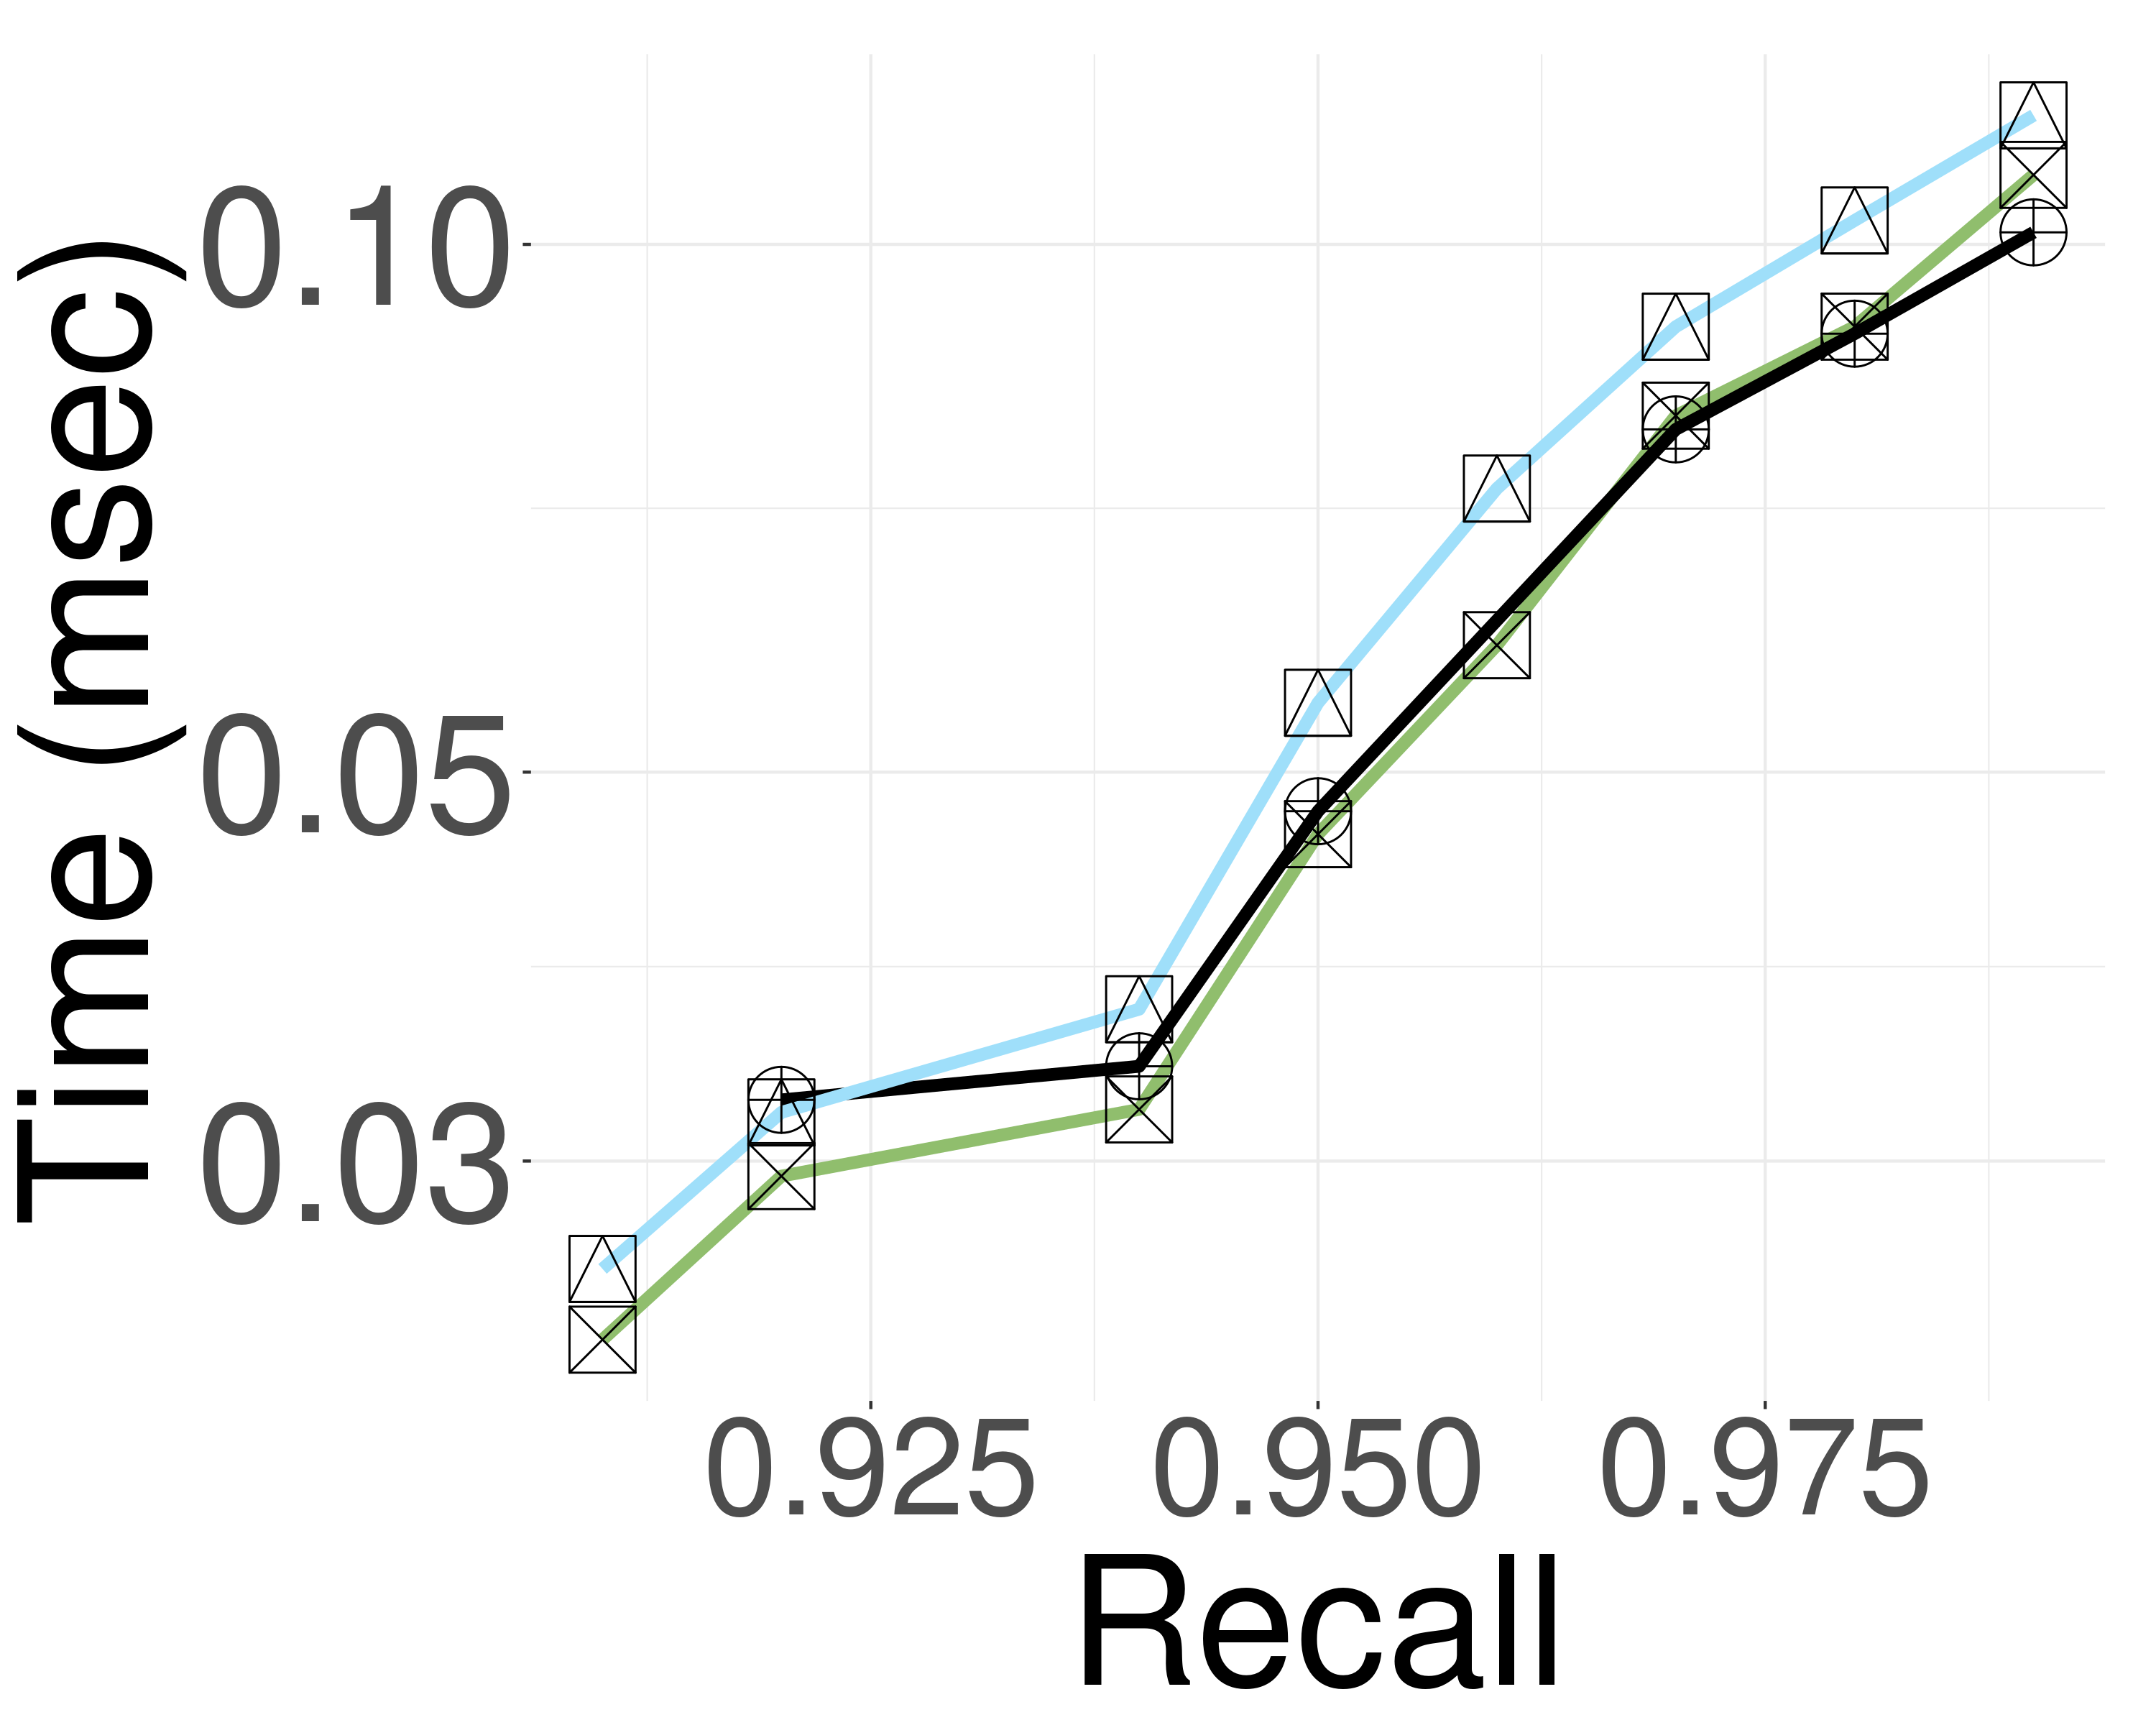
\includegraphics[width=\textwidth]{../img/elpis2/EM/1B/deep_Time.png}
			\caption{Deep}  
		\label{fig:elpisem:query:performance:1B:deep:10NN}
		\end{subfigure}
  \hspace{0.4cm}
		\begin{subfigure}{0.3\textwidth}
			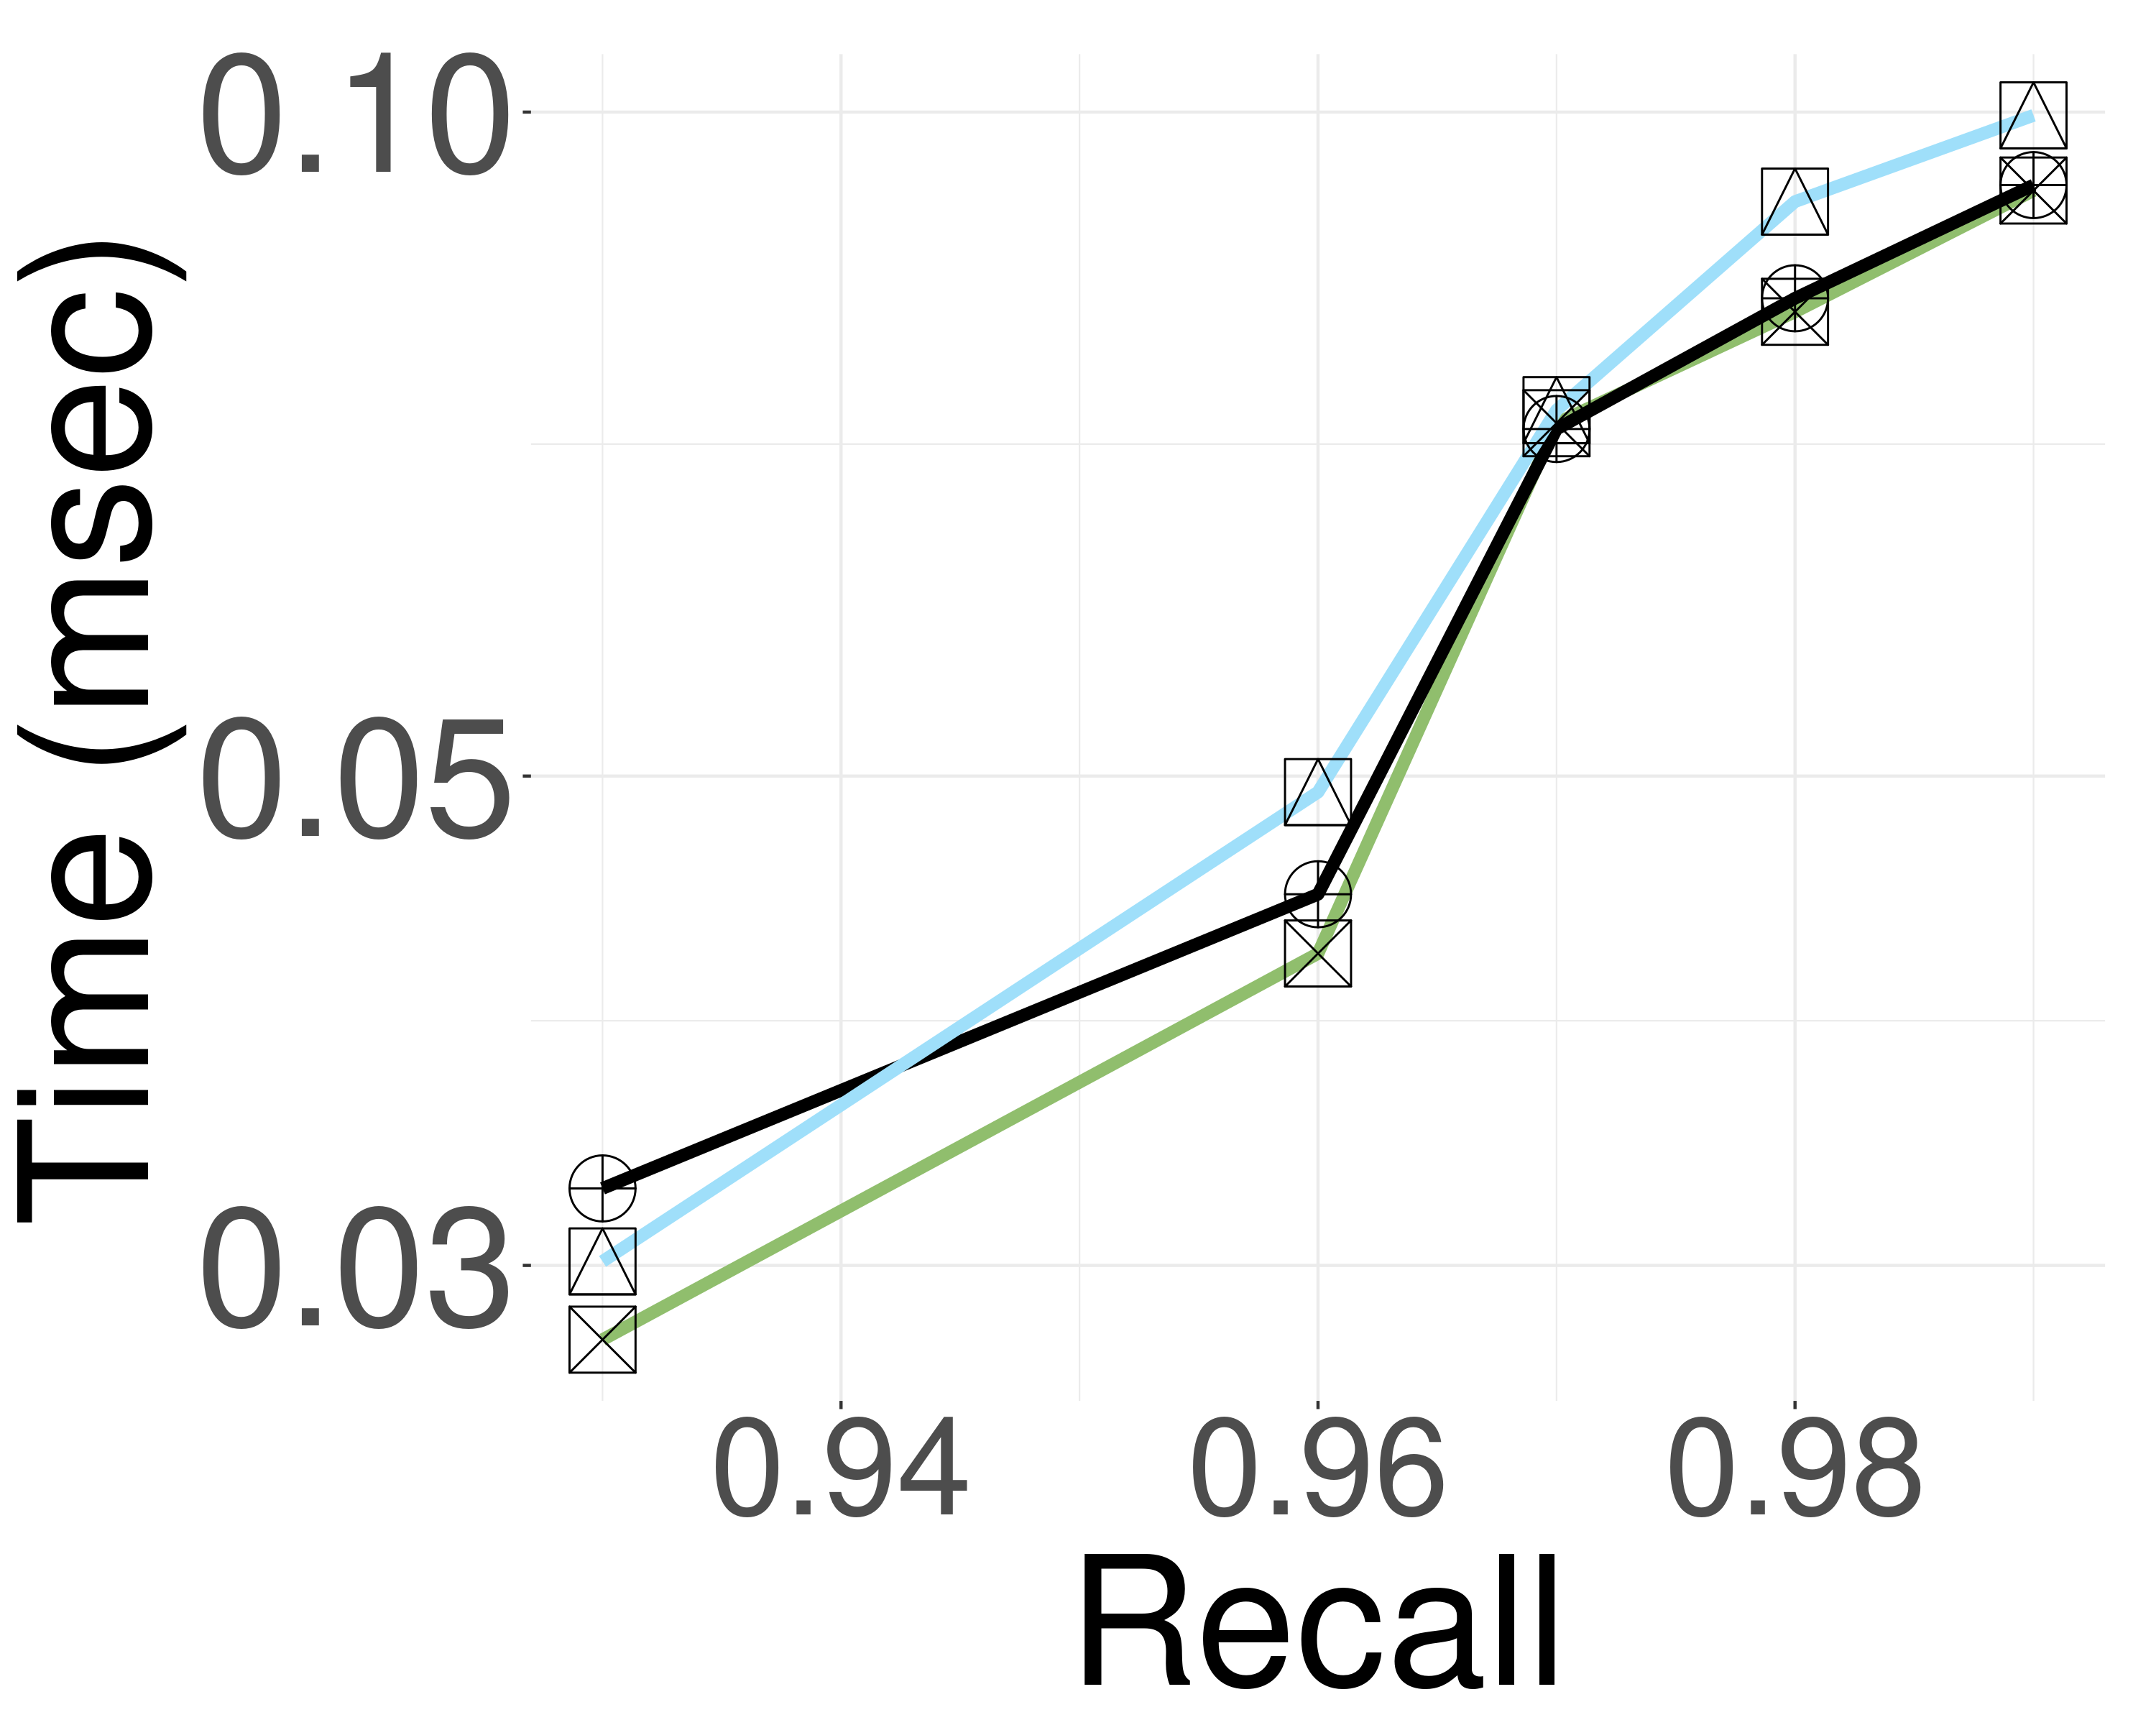
\includegraphics[width=\textwidth]{../img/elpis2/EM/1B/sift_Time.png}
			\caption{Sift}  
			\label{fig:elpisem:query:performance:1B:sift:10NN}
		\end{subfigure}
		\caption{{Search Performance on 1B datasets}}	
		\label{fig:elpisem:query:performance:1B}
	\end{figure}

 
It is worth noting that EAPCA-based merging of ELPIS can take up to 60\% less time compared to building the index with a new maximum leaf size, especially if we use pre-computed lower-bounding distances during the initial construction to select promising vertices for merging from each old leaf, thereby avoiding recomputation of these distances. This approach enables efficient adaptation to the throughput regime of the original ELPIS, which is optimized mainly for latency. Another interesting use case for EAPCA-based merging is during parameter tuning. Finding the right leaf size can become a significant disadvantage of ELPIS compared to HNSW, since the latter requires the same parameters as HNSW (M and efConstruction), in addition to an extra parameter which is the maximum leaf size. By leveraging efficient merging of leaves, we can speed up the tuning of the maximum leaf size and find the optimal value for this parameter without constructing the entire index for each leaf size choice.

While the ELPIS EAPCA-based merging strategy works well in datasets of size 100GB and below,  it is not as effective on billion-scale data collections. Designing a merging strategy that scales to very large datasets is part of our future work.

